\documentclass[a4paper,12pt,american]{scrbook} 
 
\usepackage{times}
\usepackage{mathptmx}

\usepackage[utf8]{inputenc} 
\usepackage{utf8math}

\usepackage{mathrsfs}
\usepackage[american]{babel}
\usepackage{mathtools} % includes amsmath
\usepackage{amssymb}
\usepackage{amsthm}
\usepackage{amscd}
\usepackage{todonotes}

%\usepackage{multirow}
\usepackage{enumerate}

%\usepackage{tikz}
\usepackage{framed}
%\usepackage[colorlinks]{hyperref}
%\usepackage{showlabels}  


%\usetikzlibrary{calc}
%\usetikzlibrary{intersections}
%\usetikzlibrary{arrows}
%\usetikzlibrary{decorations.pathmorphing}

\newcommand{\E}{\mathbb{E}}
\newcommand{\N}{\mathbb{N}}
\newcommand{\Q}{\mathbb{Q}}
\newcommand{\R}{\mathbb{R}}
\newcommand{\Z}{\mathbb{Z}}
\newcommand{\C}{\mathbb{C}}
\newcommand{\K}{\mathbb{K}}
\newcommand{\x}{\mathbf{x}}
\newcommand{\y}{\mathbf{y}} 
\newcommand{\X}{\mathscr{X}}
\newcommand{\cA}{\mathcal{A}}
\newcommand{\cD}{\mathcal{D}}
\newcommand{\cI}{\mathcal{I}}
\newcommand{\cP}{\mathcal{P}}
\newcommand{\cV}{\mathcal{V}}
\newcommand{\pscal}[1]{\langle {#1} \rangle}
\newcommand{\con}[1]{\overline{#1}}
\newcommand{\wt}[1]{\widetilde{#1}}
\newcommand{\car}{\mathrm{Char}}

\providecommand{\one}{\mathbf{1}}
\DeclareMathOperator{\gal}{Gal}
\DeclareMathOperator{\vol}{vol}
\DeclareMathOperator{\cont}{cont}
\DeclareMathOperator{\rank}{rang}
\DeclareMathOperator{\noy}{noyau}
\DeclareMathOperator{\cone}{cone}
\DeclareMathOperator{\tcone}{tcone}
\DeclareMathOperator{\conv}{conv}
\DeclareMathOperator{\spec}{spec}
\DeclareMathOperator{\cof}{cof}
\DeclareMathOperator{\diam}{diam}
\DeclareMathOperator{\sign}{sgn}
\DeclareMathOperator{\poly}{poly}
\DeclareMathOperator{\Ker}{Ker}
\DeclareMathOperator{\Var}{Var}
\DeclareMathOperator{\Id}{Id}
\DeclareMathOperator{\tr}{tr}
\DeclareMathOperator{\relint}{relint}
\DeclareMathOperator{\spa}{span}
\DeclareMathOperator{\Tr}{Tr}
\DeclareMathOperator{\diag}{diag}
\DeclarePairedDelimiter\mnorm{\lvert\lvert\lvert}{\rvert\rvert\rvert} % matrix norm



\theoremstyle{plain}
\newtheorem{theorem}{Theorem}[chapter]
\newtheorem{lemma}[theorem]{Lemma}
\newtheorem{proposition}[theorem]{Proposition}
\newtheorem{claim}[theorem]{Claim}
\newtheorem{corollary}[theorem]{Corollary}

\theoremstyle{definition}
\newtheorem{definition}{Definition}[chapter]
\newtheorem*{notation}{Notation}
\newtheorem{example}{Example}[chapter]
\newtheorem{remark}[theorem]{Remark}
\newtheorem{problem}{Problem}[chapter]
\newtheorem{exercise}{Exercise}[chapter]
\newtheorem{algorithm}{Algorithm}[chapter]



\newcommand{\iunit}{\mathrm{i}}
\newcommand{\CC}{{\mathbb C}}
\newcommand{\EE}{{\mathbb E}}
\newcommand{\FF}{{\mathbb F}}
\newcommand{\KK}{{\mathbb K}}
\newcommand{\NN}{{\mathbb N}}
\newcommand{\QQ}{{\mathbb Q}}
\newcommand{\RR}{{\mathbb R}}
\newcommand{\ZZ}{{\mathbb Z}}

\newcommand{\calB}{{\mathcal B}}


%opening

\title{Galois Theory }
\subtitle{MATH-317}
\author{Friedrich Eisenbrand}

%\includeonly{chapter02-theoreme-spectral}

\begin{document} 

\maketitle

\subsection*{What this course is about}
Let $E ⊇ F$ be an extension of fields. Galois theory studies the group of automorphisms $θ: E → E$ that \emph{fix} $F$. For certain extensions that are in the focus of this course, there is a remarkable connection between this group and the subfields of $E$ that contain $F$. This   \emph{Galois correspondence} enables us to  prove that the general quintic does not have a solution that is a radical expression of the coefficients.

Galois theory is an essential part of mathematical training for more than a century now. Numerous books exist that treat the subject, some of which belong to the finest writing in mathematics, see for example~\cite{van1950moderne,artin1942galois,nicholson2012introduction}. In this course,  will also discuss algorithmic aspects of Galois Theory that are not yet reflected in the canonical textbooks. We will consider the problem of calculating the Galois group of a polynomial and questions like how to transition between rational approximations of an algebraic number to its minimal polynomial via lattice basis reduction, in particular the method developed in~\cite{kannan1988polynomial}. We will also discuss the efficient algorithm for the problem to find a root of a rational polynomial in radicals~\cite{landau1985solvability}.



 \subsection*{Acknowledgments}
  The following people have helped with comments, suggestions and corrections





 \tableofcontents


 \chapter{Preliminaries}
\label{cha:preliminaries}


We assume the reader to be familiar with the content of the course \emph{MATH-215, Rings and Fields}. In the following, we briefly review some of the most important notions from this course.

Throughout this course, we assume that a ring $(R,+,⋅)$ to be commutative with \emph{unity}  $1_R \neq 0_R$. A \emph{zero divisor} is an element $a≠0$ such that there exists  an element $b≠0$ with $a⋅b = 0$. A ring without zero divisors is an  \emph{integral domain}. The \emph{characteristic} of $R$ is the order of $1$ in the additive subgroup $(R,+)$, if this order is finite. If this order is infinite, then the characteristic of is $R$ zero. The characteristic of an integral domain is either zero or a prime number.
\begin{quote}
  \small Indeed, if the order of $1$ is $m ≥1$ and if $m = p⋅q$ with natural numbers $p,q >1$, then $ p ⋅1≠ 0$ and   $q ⋅1≠0$ but  $ (p ⋅1 ) (q ⋅1) = (p⋅q) 1 = 0$ contradicting the assumption that $R$ does not contain zero divisors. 
\end{quote}


An element $u ∈ R$ is a  \emph{unit}, if there exists an element $u^{-1} ∈R$ with $u ⋅ u^{-1} = 1$. 
A \emph{field} is a ring $R$ in which $(R \setminus \{0\}, ⋅)$  is a group, or in other words, if each element of $R$ apart from $0$ is a unit. The \emph{field of quotients} of an integral domain is the set of equivalence classes of $X = \{ (r,u) : r,u ∈R, u ≠0\}$ of the equivalence relation
$  (r,u) ≡ (r',u') \quad \text{ if  and only if } r ⋅ u' = r' ⋅ u$,  together with the obvious well defined operations $+, ⋅$.




\section{Homomorphisms and ideals}
\label{sec:homomorphisms-ideals}


If $R_1$ and $R_2$ are rings, a map  $θ: R_1 → R_2$ is a \emph{ring  homomorphism} if for all $r,s ∈R_1$:
\begin{enumerate}
\item $θ(r+s) = θ(r) + θ(s)$
\item $θ(rs) = θ(r) θ(s)$
\item $θ(1_{R_1}) = 1_{R_2} $ 
\end{enumerate}
If $θ$ is a bijection, then it is a \emph{(ring) isomorphism} and we write $R_1 ≅ R_2$. If in addition $R_1 = R_2$, then $θ$ is called an \emph{automorphism}. 

If $A$ is an additive subgroup of $R$, then $R$ is partitioned into classes
\begin{displaymath}
  r + A = \{ r+a : a ∈A\}, \quad \text{ where } r ∈R. 
\end{displaymath}
Since $(R,+)$ is abelian, $A$ is a normal subgroup which makes the addition operation on classes
\begin{equation}\label{eq:1}
  (r + A ) + (s + A) = (r+s) + A
\end{equation}
well defined. We would like to have a well defined multiplication as well. 
An additive subgroup of $A$ of $R$ is an \emph{ideal} if $ra ∈ A$ for each $r∈R$ and $a ∈A$.
\begin{quote}
  \small  We repeat the argument that shows  why the multiplication~\eqref{eq:1} is well defined if and only if the additive subgroup $A$ is an ideal of $R$. If $A$ is an ideal, $r+A = r'+A$ and $s +A = s'+A$, then we need to show that $rs - r's' ∈ A$. But
  \begin{eqnarray*}
    rs - r's' & = & rs - rs' + rs' - r's' \\
              & = & r(s-s') + (r - r') s' 
  \end{eqnarray*}
  and this is an element of $A$ since both $s-s' ∈A$ and $r-r' ∈A$, as the corresponding cosets are equal.

Suppose next that the multiplication is well defined and let $r ∈R$ and $a ∈A$. Then $a+A = 0+A$ and thus the coset $ra +A$ is the coset $r⋅0 +A$  which is equivalent to $ra ∈A$. \qed
\end{quote}

We have the following theorem.
\begin{theorem}
  \label{thr:1}
  Let $A$ be an ideal of the  ring $R$. The additive factor group $R / A$ is, together with the multiplication $(r+A ) (s+A) = rs+A$ a ring with unity $1+A$.   This ring $R/A$ is called the \emph{factor ring} of $R$ by $A$.
\end{theorem}
\begin{proof}
  Since $(R,+)$ is abelian, $R/A$ is an abelian group. The multiplication is well defined and it is easy to see that $1 +A$ is the unity. Verification that the multiplication is associative and that the distributive laws hold are an exercise. 
\end{proof}

The kernel of a homomorphism $θ: R_1 → R_2$, $\ker(θ) = \{ r ∈ R_1 :θ(r) = 0\}$ is an ideal of $R_1$. If we denote the image of $θ$ by $θ(R_1) = \{ θ(r) :r ∈R_1\} ⊆ R_2$, then we can note the isomorphism theorem.
\begin{theorem}[Isomorphism theorem]
  \label{thr:2}
  Let $θ:R_1 →R_2$ be a ring-homomorphism and $A = \ker(θ)$. Then $θ$ induces the ring isomorphism $φ:R_1 / A → θ(R_1)$ with $φ(r +A) = θ(r)$. 
\end{theorem}


An ideal $P$ of a ring $R$ is called a \emph{prime ideal} if, $P ≠R$ and $P$ has the following property: If $rs ∈P$, the $r ∈P$ or $s ∈P$. One immediately has the following theorem. 

\begin{theorem}
  \label{thr:3}
  An ideal $P ≠R$ of a ring $R$ is a prime ideal if and only if $R/P$ is an integral domain. 
\end{theorem}

An ideal $M$ of $R$ is called \emph{maximal ideal}, if $M ≠R$ and the following property holds: An ideal $A$ of $R$ with $M ⊆ A ⊆R$ is either equal to $M$ or equal to $R$. One immediately has the following theorem.

\begin{theorem}
  \label{thr:4}
  Let $M$ be an ideal of $R$. Then $M$ is maximal if and only if $R/M$ is a field. 
\end{theorem}
\begin{proof}
  \small Indeed, if $M$ is maximal and $r ∉ M$, then $Rr + M$ is also an ideal that contains $M$ but is not equal to $M$ and thus is equal to $R$ and thus contains $1$. This means that there exists $x ∈R$ and $m ∈M$ with $xr + m =1$ which shows that $x+M$ is the multiplicative inverse of $r+M$. If on the other hand $R/M$ is not a field, then there exists a non-invertible element $r + M ≠ 0+M$ of $R/M$. The ideal $Rr + M$ contains $M$ strictly, but is not equal to $R$, which contradicts the fact that $M$ is maximal. 
\end{proof}


\begin{theorem}[Chinese Remainder Theorem] 
  \label{thr:8}
  Let $A$ and $B$ be ideals of a ring $R$ such that $A+B = R$ holds. Then
  \begin{displaymath}
    R/(A ∩B) ≅ R/A × R/B. 
  \end{displaymath}    
\end{theorem}
{ \small \noindent Clearly, $A∩B$ is an ideal of $R$. 
The proof is by the isomorphism theorem~\ref{thr:2} since the kernel of $φ: R →  R/A × R/B$, with $φ(r) = (r+A, r+B)$ is $A ∩B$ and since $φ$ is onto. In fact, let $1 = a+b$ with $a ∈A$ and $b∈B$, then $(x+A,y+B)$ is the image of $x⋅b + y⋅a$. 
}
\subsection*{Exercises}


\begin{enumerate}
\item Let $θ: R_1 → R_2$ be a ring homomorphism. Show that $\ker(θ) = \{ r ∈ R_1 :θ(r) = 0 \}$ is an ideal of $R_1$. 
\item Let $R$ be an integral domain and consider the construction of the field  of quotients as described above. We denote the equivalence class of $(r,u)$ with $u ≠0$ by $\frac{r}{u}$. Show that addition and multiplication
  \begin{displaymath}
    \frac{r}{u} + \frac{x}{y} = \frac{ry + ux}{uy} \quad  \text{ and } \quad  \frac{r}{u} ⋅ \frac{x}{y} = \frac{rx}{uy} 
  \end{displaymath}
  where $r,u,x,y ∈R$ and $uy ≠0$ are well defined. 
\item Complete the proof of Theorem~\ref{thr:1} by showing that the multiplication defined on $R/A$ is associative and that the distributive laws hold.
\end{enumerate}



\section{Polynomials}
\label{sec:polynomials}

The ring of polynomials with coefficients in $R$ is denoted by $R[x]$. If $f(x) ∈ R[x]$ is nonzero, then the highest exponent of $x$ that has nonzero coefficient is the \emph{degree} of $f(x)$. This coefficient is the \emph{leading coefficient} of $f(x)$. The polynomial $f(x)$ is called \emph{monic} if this leading coefficient is $1$. The degree of $0$ is not defined.  We recall division with remainder. 
\begin{theorem}
  \label{thr:5}
  Let $R$ be a ring and $f(x),g(x)∈R[x]$, $g(x) ≠0$  be polynomials such that the leading coefficient of $g$ is a unit in $R$. Then there exist uniquely determined polynomials $q(x)$ and $r(x)$ such that
  \begin{enumerate}[i)]
  \item $f(x) = q(x) g(x) + r(x)$, and
  \item either $r(x) = 0$ or $\deg r(x) < \deg g(x)$.
  \end{enumerate}
\end{theorem}
%
In particular, division with remainder implies the so-called \emph{factor theorem}. for $f(x) ∈ R[x]$ and $a ∈R$, if $f(a) = 0$, then there exists $q(x) ∈ R[x]$ with
\begin{displaymath}
  f(x) = (x - a) q(x). 
\end{displaymath}
In this case, $a$ is a \emph{root} of $f(x)$. The \emph{multiplicity} of the root $a$ is the largest $m≥1$ such that $f(x) = (x-a)^m \, g(x)$.

In the following, let $F$ denote a field. A nonzero polynomial $p(x) ∈ F[x]$ is called an \emph{irreducible polynomial}, if
\begin{enumerate}[(1)]
\item $\deg p(x) ≥1$, and
\item if $p(x) = f(x) g(x)$ with $f(x),g(x) ∈ F[x]$, then either $f(x) ∈ F$ or $g(x) ∈F$. 
\end{enumerate}
In particular, irreducible polynomials in $F$ have no root in $F$.
The \emph{content} of a polynomial $f(x) = a_0 + a_1 x + \cdots + a_n x^n ∈ Z[x]$  with integer coefficients is defined as $\cont(f) = \gcd(a_0,\dots,a_n)$. 

\begin{theorem}[Gauss's Lemma]
  Let $f(x),g(x), h(x) ∈ℤ[x]$ be nonzero polynomials with $f(x) = g(x) h(x)$, then
  \begin{displaymath}
    \cont (f) = \cont (g) \cont (h).  
  \end{displaymath}
\end{theorem}

\begin{proof}[Sketch of proof] 
  \small It suffices to show that in the case $\cont(g)  = \cont(h) =1$. Let $p$ be a prime dividing each coefficient of $f$. Write $g(x) = a_0 + a_1 x + \dots$ and $h(x) = b_0 + b_1 x + \dots$ and let $i,j$ be the smallest indices such that $p$ does not divide $a_i$ and $p$ does not divide $b_j$  respectively. The coefficient of $x^{i+j}$ in $f(x)$ is $a_ib_j + a_{i-1}b_{j+1} + a_{i-2}b_{j+2}+ \dots + a_{i+1}b_{j-1} + a_{i+2} b_{j-2}+ \dots$. Since $p$ divides this coefficient, it follows that $p$ divides $a_i$ or $p$ divides $b_j$, a contradiction. 
\end{proof}
The consequence is that a nonzero polynomial $f(x) ∈ ℤ[X]$ is irreducible in $ℚ[x]$ if and only if it cannot be written as $f(x) = g(x) h(x)$ where $g(x),h(x) ∈ ℤ[x]$ are non-constant polynomials.

\begin{theorem}[Eisenstein criterion]
  Let $f(x) = a_0 + a_1 x + \dots + a_n x^n ∈ ℤ[x]$ be a polynomial with integral coefficients, where $n≥1$.  If  there exists a prime number $p$ such  that
  \begin{enumerate}[(1)]
  \item $p$ divides $a_0,\dots,a_{n-1}$,
  \item $p$ does not divide $a_n$, and
  \item $p^2$ does not divide $a_0$, 
  \end{enumerate}
  then $f(x)$ is irreducible in $ℚ[x]$.   
\end{theorem}
\begin{proof}[Sketch of proof] 
Suppose $f(x)$ is not irreducible. Then there exist non constant polynomials $g(x) = b_0+ b_1x + \dots + b_rx^r ∈ℤ[x]$ and $h(x) = c_0+ c_1x+ \dots + c_sx^s ∈ℤ[x]$ such that $f(x) = g(x) h(x)$. The prime $p$ divides either $b_0$ or $c_0$. Assume it divides $c_0$. Let $0<i<s$ be the first index such that $p$  does not divide $c_i$. The coefficient of $x^i$ in $f(x)$ is $b_0c_i + b_1c_{i-1}+ \dots$. This implies $p$ divides $c_i$.  
\end{proof}

The Eisenstein criterion is sufficient but not necessary for irreducibility. How can we rigorously test whether $f(x) = a_0 + a_1 x + \dots a_n x^n ∈ ℤ[x]$  is irreducible? One way to do so is to derive bounds on the coefficients of a possible factor, see~\cite{mignotte1974inequality}.

We define the \emph{norm} of a complex polynomial  $f(x) = a_0+a_1x+ \cdots+a_nx^n ∈ ℂ[x]$ by  $\|f\|_2 = \sqrt{∑_{i=0}^n |a_i|^2}$ where $|⋅|$ denotes the usual norm in $ℂ$. By the fundamental theorem of algebra, we can write
\begin{displaymath}
f(x)  = a_n ∏_{i=1}^n (x-z_i),  
\end{displaymath}
where the $z_i$ are the roots of $f(x)$. We define the \emph{measure} of $f(x)≠0$ as
\begin{displaymath}
  M(f) = |a_n| ∏_{i=1}^n \max\{1,|z_i|\},
\end{displaymath}
and $M(0) = 0$. 
Clearly, the measure is multiplicative, i.e., for $f(x),g(x) ∈ℂ[x]$ are nonzero, then
\begin{displaymath}
  M(f(x)g(x)) = M(f(x)) \, M (g(x)). 
\end{displaymath}


The next assertion bounds the norm of $f(x)$ by the measure $M(f)$ from above. To this end, we also introduce the $1$-norm of a polynomial $f(x) = a_0+ \cdots+a_nx^n∈ ℂ[x]$ as
\begin{displaymath}
  \|f\|_1 = ∑_{i=0}^n |a_i| 
\end{displaymath}
and recall $\|f(x)\|_2 ≤ \|f(x)\|_1$. 

\begin{theorem}
  \label{thr:6}
  Let $f(x) =a_0 + \cdots + a_n x^n∈ ℂ[x]$, then $\|f(x)\|_1 ≤ 2^n M(f(x))$. 
\end{theorem}
\begin{proof}
  Let us denote the roots of $f(x)$ by $z_1,\dots, z_n$. Then
  \begin{displaymath}
    f(x) = a_n ∏_{i=1}^n (x-z_i).
  \end{displaymath}
  The $i$-th coefficient of $f(x)$ is
  \begin{displaymath}
    a_i = (-1)^{n-i} a_n  ∑_{ S ∈ \binom{n}{n-i}} ∏_{j ∈S} z_j. 
\end{displaymath}
This implies
\begin{displaymath}
  |a_i| ≤ \binom{n}{n-i} M(f(x)) 
\end{displaymath}
and thus
\begin{displaymath}
  ∑_{i=0}^n |a_i| ≤ 2^n M(f(x)) 
\end{displaymath}
follows. 
\end{proof} 
%
\begin{lemma}
  \label{lem:1}
  For $f(x) ∈ℂ[x]$ and $z ∈ℂ$, one has
  \begin{displaymath}
    \|(x-z) f(x)\|_2 = \|(\overline{z}x-1) f(x)\|_2. 
  \end{displaymath}
\end{lemma}
\begin{proof}
  If we define $a_{-1}=0$ and $a_{n+1} = 0$, then
  \begin{eqnarray*}
    \|(x-z) f(x)\|_2^2 & = & ∑_{i=0}^{n+1} | a_{i-1} - z a_i|^2 \\
                       & = & ∑_{i=0}^{n+1} (a_{i-1} - z a_i) (\con{a_{i-1}} - \con{z} \con{ a_i})  \\
                      & = & (1+ |z|^2 ) \|f(x)\|_2^2 - ∑_{i=0}^{n+1} \con{z} a_{i-1} \con{a_{i}} + z \con{a_{i-1}} a_i . 
  \end{eqnarray*}
%
Similarly, we develop
  \begin{eqnarray*}
    \|(\con{z}x-1) f(x)\|_2^2 & = & ∑_{i=0}^{n+1} | \con{z} a_{i-1} -  a_i|^2 \\
                       & = & ∑_{i=0}^{n+1} (\con{z} a_{i-1} -  a_i) (z \con{a_{i-1}} -  \con{ a_i})  \\
                      & = & (1+ |z|^2 ) \|f(x)\|_2^2 - ∑_{i=0}^{n+1} \con{z}  a_{i-1}\con{a_{i}} + {z}  \con{a_{i-1}} a_i. 
  \end{eqnarray*}
\end{proof}
%
We next want to bound the norm by the measure from below.
%
\begin{theorem}[Landau's inequality]
  Let $f(x) ∈ℂ[x]$, then $M(f) ≤ \|f(x)\|_2$. 
\end{theorem}
\begin{proof}
  This clearly holds for the zero polynomial. Thus, let $f(x)≠0$ and suppose the roots $z_i$ are ordered such that $|z_1|,\dots,|z_k| >1$ and $|z_{k+1}|,\dots,|z_n| ≤1$ such that $M(f) = |a_n ⋅ z_1 \cdots z_k|$. We define the polynomial
  \begin{displaymath}
    g(x) = a_n ∏_{j=1}^k (\con{z_j}x-1) ∏_{i=k+1}^n(x-z_i) = g_n x^n + \cdots + g_0 ∈ ℂ[x]. 
  \end{displaymath}

  One has
  \begin{eqnarray*}
    M(f)^2 &=& |g_n|^2 \\
           & ≤& \|g(x)\|_2^2 \\
           & = & \| \frac{g(x)}{\con{z_1}x-1} (x-z_1) \|_2^2\\
           & = & \| \frac{g(x)}{(\con{z_1}x-1) \cdots (\con{z_k}x-1)} (x-z_1) \cdots  (x-z_k) \|_2^2 \\
           & = & \|f(x)\|_2^2,  
  \end{eqnarray*}
  where we applied Lemma~\ref{lem:1} repeatedly.    
\end{proof}

\begin{theorem}
  \label{thr:7}
  Let $f(x) ∈ ℤ[x]$ be a nonzero polynomial of degree $n$ and $g(x),h(x) ∈ℤ[x]$ with
  $f(x) = g(x) h(x)$, then
  \begin{displaymath}
    \|g\|_1 ≤ 2^n \|f\|_2. 
  \end{displaymath}    
\end{theorem}

\begin{proof}
  Theorem~\ref{thr:6} implies    $\|g\|_1 ≤ 2^n M(g)$. Since the measure is multiplicative and the coefficients are all integral, the absolute value of the leading coefficient of $f$ is at least the one of $g$ and therefore $M(g) ≤ M(f)$. Finally Landau's inequality yields $M(f)≤ \|f\|_2$. This yields
  \begin{displaymath}
    \|g\|_1 ≤ 2^n \|f\|_2. 
  \end{displaymath}
\end{proof}



Theorem~\ref{thr:7} enables us to solve the problem whether a given polynomial $f(x) ∈ℤ[x]$  with content $1$ is irreducible or not with a finite algorithm. The assertion states that a factor $g(x) ∈ℤ[x]$ satisfies $\|g\|_1 ≤ 2^n \|f\|_2$, where $n$ is the degree of $f$. We can simply list all polynomials of degree at most $n$ that satisfy this bound. This is a finite but not efficient algorithm. It is exponential in the degree and in the binary encoding length of the largest absolute vallue of a coefficient of $f$. The problem has an efficient algorithmic solution. This is a celebrated result by Lenstra, Lenstra and Lovàsz~\cite{lenstra1982factoring}.  


\subsection*{Exercises}
\begin{enumerate}
\item Let $f(x) ∈ R[x]\setminus\{0\}$ and $a ∈R$ be a root of $f(x)$ with multiplicity $m$. Let $g(x) ∈ R[x] $ with $f(x) = (x-a)^m g(x)$. Show that $a$ is not a root of $g(x)$.
\item Let $R$ be an integral domain and  $f(x) ∈ R[x]$ be a nonzero polynomial. Show that $f(x)$ has at most $\deg f(x)$ many different roots.
\item Describe an irreducible (in $ℚ[x]$) polynomial $p(x) ∈ℤ[X]$ with degree at least two which does not satisfy the Eisenstein criterion.
\item Let  $f(x),g(x) ∈ℂ[x]$ be nonzero. Show that $M(f(x)g(x)) = M(f(x)) \, M (g(x))$.
\item Let $f(x),g(x) ∈ℂ[x]$ be nonzero polynomials with leading coefficients $a,b ≠0$ where $\deg (f) = n$ and where $g$ divides $f$. Show the following generalization of Theorem~\ref{thr:7}: $\|g\|_1 ≤ 2^n |b| / |a| \|f\|_2$. 
\end{enumerate}


% \subsection{Polynomials over a field}
%\label{sec:polyn-with-coeff}

In the following, let $K$ be field. The polynomial ring $K[x]$ is a \emph{euclidean domain} and therefore a \emph{principal ideal domain} and consequently a \emph{unique factorization domain}, this means that a factorization of $f(x)$ into \emph{monic} (leading coefficient equal to one) irreducible polynomials $p_i(x)$  and $α ∈K$ 
\begin{equation}
  \label{eq:3}
  f(x) = α p_1(x) \cdots p_k(x), 
\end{equation}
is unique up to the ordering of the $p_i(x)$. Recall that an ideal $A$ of a ring  $R$  is called \emph{principal} if it is of the form $A = \{ r a : r ∈R\}$ for some $a ∈A$. For $a_1,\dots,a_k ∈R$, the set  $\{ r_1 a_1+ \cdots + r_k a_k : r_i ∈R, \, i=1,\dots,k\}$ is called the \emph{ideal generated by} $a_1,\dots,a_k$ and it is  denoted by $〈a_1,\dots,a_k〉$. 

It is easy to see that a nonzero ideal $A$ of $K[x]$ is principal. In fact, one chooses simply an element $g(x) ∈A \setminus \{0\}$ of minimal degree. If $f(x) ∈A$, then we perform division with remainder
\begin{displaymath}
  f(x)  = q(x) g(x) + r(x) 
\end{displaymath}
from which $r(x) ∈A$ follows and since $g(x)$ is the non-zero  element of smallest degree of $A$, one has $r(x) = 0$, meaning that $g(x)$ divides $f(x)$ and thus $A = 〈g(x)〉$.

From this one can conclude the following important fact from which the uniqueness of the factorization~\eqref{eq:3} follows. (Existence is in fact almost trivial.)
\begin{theorem}
  \label{thr:9}
  Let $p(x) ∈K[x]$ be irreducible and suppose that $p(x)$ divides $f(x) ⋅ g(x) ∈ K[x]$. Then $p(x)$ divides $f(x)$ or $p(x)$ divides $g(x)$. 
\end{theorem}
{\small \noindent 
  In fact, if $p(x)$ does not divide $f(x)$, then $〈p(x),f(x)〉 = 〈1〉$ which means that there are $h_1(x), h_2(x) ∈ K[x]$ with $1 = h_1(x) p(x) + h_2(x) f(x)$. But then
  \begin{equation}
    \label{eq:2}
    g(x) = h_1(x) p(x)  g(x)+ h_2(x) f(x) g(x),
  \end{equation}
  and since $p(x)$ divides $f(x) ⋅g(x)$ the term on the right of~\eqref{eq:2} is divisible by $p(x)$ and thus $h(x)$ is divisible by $p(x)$. \qed
  
}


Given $f(x),g(x) ∈K[x]$, not both zero, we now recall how to compute $h(x) ∈ K[x]$ with
\begin{displaymath}
  〈h(x) 〉 = 〈 f(x),g(x) 〉. 
\end{displaymath}
A polynomial $d(x) ∈K[x]$ that divides both $f(x)$ and $g(x)$ is a \emph{common divisor} of $f(x)$ and $g(x)$. A \emph{greatest common divisor} of $f(x)$ and $g(x)$ is a common divisor of $f(x)$ and $g(x)$ that is divided by any common divisor of $f(x)$ and $g(x)$.  If one requires the greatest common divisor to be monic, then it is also unique. It is the product of the common irreducible factors of $f(x)$ and $g(x)$ in~\eqref{eq:3}.

We can efficiently compute the greatest common divisor of two polynomials $f_0(x), f_1(x) ∈ K[X]$ where $f_0(x) ≠0$   with the Euclidean algorithm, that computes the reminder sequence
\begin{displaymath}
  f_0(x),f_1(x),\dots,f_k(x), 
\end{displaymath}
where
\begin{equation}
  \label{eq:4}
  f_{i-1}(x) = q_i(x) f_i(x) + f_{i+1}(x)
\end{equation}
is the result of dividing $f_{i-1}(x)$    by $f_i(x)$ with remainder $f_{i+1}(x)$ for $i=1,\dots,k-1$. The polynomial $f_k(x) = 0$ is the first remainder that is zero, i.e.,  $f_i(x) ≠0$ for $i=0,\dots,k-1$. Clearly, the set of common divisors of $f_{i-1}(x)$ and $f_i(x)$  is the set of common divisors of $f_{i}(x)$ and $f_{i+1}(x)$ in~\eqref{eq:4}. This means that the greatest common divisor of $f_0(x)$ and $f_1(x)$ is $f_{k-1}(x)$. inspecting the remainder sequence, one observes further that
\begin{equation}
  \label{eq:5}
  \begin{pmatrix}
    f_{i} \\
    f_{i+1}
  \end{pmatrix}
  =
  \begin{pmatrix}
    0 & 1 \\
    1 & -q_i
  \end{pmatrix}
  \begin{pmatrix}
    f_{i-1}  \\
    f_{i}
  \end{pmatrix}
\end{equation}
and thus
\begin{equation}
  \label{eq:6}
   \begin{pmatrix}
    f_{k-1} \\
    f_{k}
  \end{pmatrix}
  =
  U 
  \begin{pmatrix}
    f_0  \\
    f_1
  \end{pmatrix}
\end{equation}
where
$
U 
  $
  is the matrix 
\begin{equation}
  \label{eq:7} U =    
  \begin{pmatrix}
    0 & 1 \\
    1 & -q_{k-1}
  \end{pmatrix} \cdots
  \begin{pmatrix}
    0 & 1 \\
    1 & -q_{1}
  \end{pmatrix}. 
\end{equation}



\begin{example}
  \label{exe:1}
  We compute the greatest common divisor of
  \begin{displaymath}
     f_0(x)= x^5 - 2x^4 + 3x^3 - 3x^2 + 1
  \end{displaymath}
  and
  \begin{displaymath}
    f_1(x) = x^4 - x^3 - x + 1.
  \end{displaymath}
    Successive division with remainder yields the sequence 
  \begin{eqnarray*}
    f_0(x) &= &  x^5 - 2x^4 + 3x^3 - 3x^2 + 1 \\
    f_1(x) &=&  x^4 - x^3 - x + 1 \\
    f_2(x) & = & 2x^3 - 2x^2 - 2x + 2 \\
    f_3(x) & = &  x^2 - 2x + 1 \\
    f_4(x) & = & 0
  \end{eqnarray*}
  with the corresponding quotients    
  \begin{eqnarray*}
    \label{eq:9}
    q_1(x) & = &  x - 1 \\
    q_2(x) & = &  \frac{1}{2}x \\
    q_3(x) & = &   2x + 2.     
  \end{eqnarray*}
The greatest common  divisor is $x^2 - 2x + 1$. The matrix $U$ is 
  \begin{eqnarray*}
    U & = &  \left(\begin{array}{rr}
0 & 1 \\
1 & -2 x - 2
\end{array}\right) ⋅
\left(\begin{array}{rr}
0 & 1 \\
1 & -\frac{1}{2} x
\end{array}\right) ⋅ 
\left(\begin{array}{rr}
0 & 1 \\
1 & -x + 1
      \end{array}\right) \\
    & = & \left(\begin{array}{rr}
-\frac{1}{2} x & \frac{1}{2} x^{2} - \frac{1}{2} x + 1 \\
x^{2} + x + 1 & -x^{3} - 2 x - 1
\end{array}\right).
  \end{eqnarray*}
  And indeed
  \begin{displaymath}
    -\frac{1}{2} x  ⋅ f_0(x) +  \left(\frac{1}{2} x^{2} - \frac{1}{2} x + 1\right) ⋅ f_1(x) = x^2 - 2x + 1. 
  \end{displaymath}
\end{example}


Let $f(x) = a_0 + a_1x + \cdots + a_n x^n ∈ F[x]$  be a polynomial. The \emph{derivative} of $f$ is the polynomial $f'(x) = a_1 + 2 a_2x + \cdots + n a_n x^{n-1}$. The following is easily verified by comparing the coefficients of the resulting polynomials. 
\begin{theorem}
  \label{thr:10}
  Let $f$ and $g$ be polynomials in $F[x]$, where $F$ is a field, then
  \begin{enumerate}[i)]
  \item $(f(x) + g(x))' = f'(x) +  g'(x)$, 
  \item $(f(x) g(x))' = f'(x)g(x)  +  f(x) g'(x)$, and
  \item $(f(g(x)))' = f'(g(x))g'(x)$. 
  \end{enumerate}
\end{theorem}



\section{Field extensions}
\label{sec:field-extensions}

Let $E$ and $F$ be fields. If $E ⊇ F$ holds, then $E$ is a \emph{field extension} of $F$. It is an important observation that $E$ is an $F$-vector space and thus the concepts of linear algebra can be used. The dimension of $E$ as an $F$ vector space is denoted by $[E:F]$. It is also called the \emph{degree of the extension}. A field extension of finite degree is also called a \emph{finite field extension}.

\begin{theorem}[Tower Law] 
  \label{thr:10}
  Let $E ⊇F$ be a finite field extension and $K$ an intermediate field, i.e.,  $E ⊇K ⊇F$, then
  \begin{displaymath}
    [E:F] = [E:K] ⋅ [K:F] 
  \end{displaymath}
\end{theorem}
The proof of the tower  law is a simple exercise in linear algebra. 

An element $α∈ E$ is \emph{algebraic} over $F$, if there exists a nonzero polynomial $f(x) ∈ F[x]$  such that $f(α)= 0 $ holds. The \emph{minimal polynomial} of $α$ is the unique monic and non-zero polynomial $p(x) ∈ F[x] $ of minimal degree with $p(α)=0$. For fields $E ⊇ F$ and $u_1,\dots,u_k ∈E$, $F(u_1,\dots,u_k)$ denotes the inclusion-wise minimal intermediate field of $E⊇F$ that contains $u_1,\dots,u_k$. We have the following important fact. If $u ∈E$ is algebraic over $F$ with minimal polynomial $p(x) = a_0+ \cdots + a_n x^n ∈F[x]$, then
\begin{equation}
  \label{eq:8}
  F(u) ≅ F[x] / 〈p(x)〉.  
\end{equation}
This follows from the isomorphism theorem~\ref{thr:2} by inspecting  ring homomorphism
\begin{equation}
  \label{eq:10}
  \begin{array}{rccc}
    φ: & F[x] &→&  E \\
       &  f(x) & ↦ & f(u). 
  \end{array}
\end{equation}
The image $φ(F[x])$ of $φ$ is isomorphic to $ F[x] / 〈p(x)〉$. Since $p(x)$ is irreducible, $〈p(x)〉$ is maximal and thus $ F[x] / 〈p(x)〉$ is a field. The image $φ(F[x])$ is clearly contained in  $F(u)$ and since the image is a field, it is equal to the smallest extension field of $F$ containing $u$, which is $F(u)$. A further consequence of this fact is Kronecker's Theorem.
\begin{theorem}[Kronecker's Theorem]
  \label{thr:11}
  If $F$ is any field and if $f(x) ∈ F[x]$ is a non-constant polynomial, then there exists a field extension of $F$ in which $f(x)$ has a root. 
\end{theorem}
The proof is by inspecting an irreducible factor $p(x)$ of $f(x)$ and by embedding $F$ into $F[x] / 〈p(x)〉$ via the injective homomorphism $π: F →F[x] / 〈p(x)〉$  defined by  $π(r) = r + 〈p(x)〉$.


\begin{definition}
  \label{def:1}
  Let $f(x)$ be a polynomial in $F[x]$ with $\deg(f) ≥1$, where $F$ is a field. An extension $E ⊇F$ is called a \emph{splitting field} of $f$ over $F$ if
  \begin{enumerate}[i)]
  \item  $f(x) = a (x-u_1) \cdots (x - u_n)$, where $a ∈F$ and $u_i ∈E$ for each $i$ and
  \item $E = F(u_1,\dots,u_n)$. 
  \end{enumerate}
\end{definition}

\begin{theorem}
  \label{thr:12}
  Let $f$ be a polynomial of degree $n≥1$ over a field $F$. Then a splitting field $E ⊇F$ of $f$ over $F$ exists and $[E:F] ≤ n!$. 
\end{theorem}
{\small \noindent 
The proof is by induction on $n$. If $n=1$,  then $E = F$ is a splitting field. This is also the case if $f(x)$ splits into linear factors over $F$ already. Otherwise, let $p(x) ∈ F[x]$ be a monic irreducible factor of $f(x)$ with $\deg(p) ≥2$.  Let $K ⊇ F$ be an extension that contains a root $u_1$ of $p$ and let $E_1 = F(u_1)$. Clearly $[E_1:F] ≤ n$ and $f(x) = (x - u_1) g(x)$ with $g(x) ∈ E_1[x]$ has degree $n-1$. By induction, there exists a splitting field $E_2 ⊇ E_1$ of $g$ and this is of the form $E_2 = E_1(u_2,\dots,u_n)$ and one has $[E_2:E_1] ≤ (n-1)!$. Clearly $F(u_1,\dots,u_n)$ is a splitting field of $f$ over $F$ of degree at most $n ⋅(n-1)! = n!$. \qed
}


The next theorem shows that splitting fields are unique up to isomorphism.

\begin{theorem}
  \label{thr:13}
  Let $π: F → \overline{F}$ be an isomorphism of fields and let $f(x) = a_0+ \dots+a_nx^n ∈ F[x]$ be a non-constant polynomial and let $f^π(x) = π(a_0)+\dots+π(a_n) x^n ∈ \overline{F}[x]$. If $E⊇F$ is a splitting field of $f(x)$ over $F$ and  $\overline{E}⊇\overline{F}$ is a splitting field of $f^π(x)$ over $\overline{F}$, then there exists an isomorphism $φ: E → \overline{E}$ that extends $π$, i.e. for which $π(r) = φ(r)$ for each $ r ∈ F$ holds. 
\end{theorem}

The proof is by induction, see diagram below. 
\begin{displaymath}
  \begin{CD}
    E @>φ>> \overline{E} \\
    @AAA     @AAA \\
    F(u) @>τ >>\overline{F}(v) \\
    @AAA     @AAA \\
     F @>π >>\overline{F}
  \end{CD}
\end{displaymath}


\begin{proof}
  First we observe that the mapping $ F[x] → \overline{F}[x]$ with $f ↦ f^π$ is a ring-isomorphism that extends $π$ (Exercise).
  Let $f(x) = p_1(x) \cdots p_k(x) ⋅ (x-a_1) \cdots (x-a_l)$ where the $p_i∈ F[x]$ are irreducibles of degree at least two and $a_i ∈F$. 
  
  The proof is then by induction on $\deg p_1 + \cdots + \deg p_k$. If this sum is equal to zero,  then $E = F$ and $\overline{E} = \overline{F}$ and the assertion obviously holds. Let $p(x)∈ F[x]$  be an irreducible factor of $f(x)$ of degree at least two and let $u ∈ E$ be a root of $p(x)$. Similarly, let $v ∈ \overline{E}$ be a root of the irreducible factor $p^π(x)$ of $f^π(x)$.

  We have argued, see~\eqref{eq:8} that $F(u) ≅ F[x] / 〈 p(x) 〉$ and $\overline{F}[x] / 〈p^π(x)〉 ≅ \overline{F}(v)$. Let $Ψ_1: F(u) → F[x] / 〈 p(x) 〉$ and $Ψ_2: \overline{F}[x] / 〈p^π(x)〉 →  \overline{F}(v)$ be the corresponding isomorphisms.   The  mapping  $Ψ_3: F[x] / 〈p(x)〉 → \overline{F}[x] / 〈p^π(x) 〉$ with 
  \begin{equation}
    \label{eq:11}
    Ψ_3 (h(x) + 〈p(x) 〉 ) = h^π(x) + 〈p^π(x)〉
  \end{equation}
  is well defined (Exercise) 
  and an isomorphism that extends $π$. Clearly $ τ = Ψ_2 \circ  Ψ_3 \circ Ψ_1: F(u) → \overline{F}(v)$ is an isomorphism extending $π$. Since $f$ has at least one linear factor more in $F(u)$ than in $F$, we can apply induction now. There exists an isomorphism $φ: E → \overline{E}$ that extends $τ$ and thus also extends $π$.       
\end{proof}


\begin{corollary}
  \label{co:1}
  Let $f(x) ∈ F[x]$ be a non-constant polynomial and $E ⊇F$ as well as $\overline{E} ⊇F$ be splitting fields of $f$ over $F$, then $E ≅ \overline{E}$. 
\end{corollary}

A polynomial $f(x) ∈ F[x] \setminus\{0\}$ is called \emph{separable}, if it does not have any multiple roots in any field extension $E ⊇F$. We can check easily, whether a polynomial $f(x) ∈F[x]$ is separable. 
\begin{theorem}
  \label{thr:14}
  A non-zero polynomial $f(x) ∈ F[x]$ is separable, if and only if $\gcd(f,f') = 1$. 
\end{theorem}

\begin{proof}
  Suppose that $f$ is separable. We show $\gcd(f,f') = 1$. This is the case if $\deg(f)≤1$ because then, either $f$ is a constant or $f'$ is a nonzero constant.   Thus suppose that $\deg(f)>1$ and that  $x-u$ divides both $f$ and $f'$, where $u$ is an element of a splitting field $E ⊇ F$. Then $f = (x-u) g$  and thus $f'= g + (x-u) g'$. This means that $(x-u)$ divides $g$ and thus that $u$ is a double root of $f$. This is a contradiction. 

  If $\gcd(f,f') = 1$, then there exist $g,h∈ F[x]$ such that $g ⋅ f + h ⋅f'=1$. This means that no polynomial $x-u$ with $u ∈E$ can divide both $f$ and $f'$ and thus $(x-u)^2$ does not divide $f$. This means that  $f$ is separable.
\end{proof}

\begin{theorem}
  \label{thr:15}
  Let $p(x) ∈ F[x]$ be irreducible. If $\car(F) = 0$, then $p(x)$ is separable. If $\car(F) = q$, then $p$ is not separable if and only if $p(x) = h(x^p)$ for some $h(x) ∈ F[x]$. 
\end{theorem}

\begin{proof}
  If $p' ≠0$ then $\gcd(p,p')=1$, since $p$ is irreducible and with
  Theorem~\ref{thr:14} it follows that
  $p$ is separable if and only if $p'≠0$. 
   This is
  the case if $\car(F) = 0$.
  
  Let $p(x) = a_0 + a_1x + \cdots + a_n x^n$ with $n≥1$ and $a_n ≠0$,
  then $p'(x) = a_1 + 2a_2x + \cdots + n ⋅ a_n x^{n-1}$. This shows that, if  $\car(F) =q$, then $p'=0$ if and only if $a_i = 0$ whenever $i ≠ 0 \pmod{q}$. This means that $f(x) = g(x^q)$ with $g(x) = a_0 + a_qx + a_{2q}x^{2} + \cdots$. 
  
\end{proof}

\begin{definition}
  Let $E ⊇F$ be a finite field extension. An element $u ∈E$ is called \emph{separable} if its minimal polynomial $p(x) ∈F[x]$ is separable. If each element of $E$ is separable, then the extension $E⊇F$ is a \emph{separable extension}. 
\end{definition}


\begin{theorem}[Primitive element theorem]
  \label{thr:16}
  Let $E ⊇ F$ be a finite field extension, $u_1,\dots,u_k ∈E$ and suppose that $u_2,\dots,u_k$ are separable. Then there exists an element $u ∈ F(u_1,\dots,u_k)$ with
  \begin{displaymath}
    F(u) =  F(u_1,\dots,u_k). 
  \end{displaymath}  
\end{theorem}

\begin{proof}
  If $F$ is a finite field, then so is  $F(u_1,\dots,u_k)$. The group of units  in a finite field is cyclic. Clearly, $F(u_1,\dots,u_k) = f(α)$, where $α$ is a generator of $(F(u_1,\dots,u_k) \setminus \{0\}, ⋅)$. To this end, let us assume that $F$ is infinite. We show the theorem  for $k=2$, i.e., we show that there exists an element $u ∈ F(u_1,u_2)$ with $F(u) = F(u_1,u_2)$. The assertion  then  follows by induction on $k$.

 


To simplify notation, we denote  $α = u_1$ and $β = u_2$. We claim that there exists an element $y ∈F \setminus \{0\}$ such that $α + yβ$ is a generator of the field extension.  Let $p(x)$ and $q(x)$ be the minimal polynomials of $α$ and $β$ respectively. We can factor
  \begin{eqnarray*}
    p(x) & = &  (x- α_1) \cdots (x-α_n)  \\
    q(x) & = & (x- β_1) \cdots (x-β_m) 
  \end{eqnarray*}
  in a splitting field of $E ⊇ F$ of $p(x)⋅q(x)$, where $α=α_1$ and $β = β_1$. The $β_i$ are pairwise different.

  For $y ∈ F$ we  define the polynomial
  \begin{equation}
    \label{eq:12}
    h_y(x) = p( (α + y β) - y ⋅ x) ∈ F(α + y β)[x]. 
  \end{equation}
  The idea is to choose $y ∈F \setminus \{0\}$ in such a way that
  \begin{equation}
    \label{eq:13}
    (x-β) =  \gcd(q,h) 
  \end{equation}
  holds.  Since $\gcd(q,h) ∈ F(α + y β)[x]$, this shows that
  $β ∈ F(α + y β)$ and therefore also $α ∈ F(α + y β)$. Consequently
  $F(α,β) = F(α + y β)$.

  We have~\eqref{eq:13} if and only if none of the elements $β_2,\dots,β_m$ are roots of $h(x)$ and this is if and only if $y ∈ F$ was chosen such that
  \begin{equation}
    \label{eq:14}
    α + y β - y β_i ≠ α_j, \, \text{ holds for } 2≤ i ≤ m, \, 1 ≤ j ≤ n.  
  \end{equation}
  For $i,j$ in this range fixed, one has
  \begin{displaymath}
     α + y β - y β_i = α_j 
   \end{displaymath}
   if and only if
   \begin{displaymath}
     y (β - β_i) = α_j - α 
   \end{displaymath}
   and since the $β≠ β_i$ this holds if and only if
   \begin{displaymath}
     y  = (α_j - α)  / (β - β_i). 
   \end{displaymath}
   This shows that any $y$ from the set
   \begin{displaymath}
     F \setminus \{ (α_j - α)  / (β - β_i) :  2≤ i ≤ m, \, 1 ≤ j ≤ n\}
   \end{displaymath}
   satisfies
   \begin{displaymath}
     F(α,β) = F(α + y β). 
   \end{displaymath}  
\end{proof}



%%% Local Variables:
%%% mode: latex
%%% TeX-master: "notes"
%%% End:

 
\chapter{Galois Groups and the Main Theorem of Galois Theory}
\label{cha:galois-groups-galois}

We now come to a central definition of this course. 

\begin{definition}
  \label{def:2}
  If $E ⊇F$ is an extension of fields, an automorphism $σ: E → E$ that satisfies $σ(a) = a$ for each $a ∈ F$ is said to \emph{fix} $F$ and it is called an \emph{$F$-automorphism}.  The set of $F$-automorphisms are, together with composition a group. It is called the \emph{Galois group} of the extension $E ⊇F$ and we denote it by $\gal(E:F)$.
\end{definition}

The next lemma is simple to prove, but very helpful in understanding the Galois group.

\begin{lemma}
  \label{lem:2}
  Let $E ⊇F$  be a field extension, $f(x) ∈ F[x]$, $τ ∈ \gal(E:F)$ and $u ∈ E$. Then $τ(f(u)) = f(τ(u))$. In particular, if $u$ is a root of $f$, then so is $τ(u)$. 
\end{lemma}
\begin{proof}
  Let $f(x)  = a_0 + a_1x + \cdots + a_n x^n ∈F[x]$, then
  \begin{eqnarray*}
    τ(f(u)) & = & τ (a_0 + a_1u + \cdots + a_n u^n) \\
            & = & τ (a_0) + τ(a_1u)  + \cdots + τ(a_n u^n) \\
            & = & τ (a_0) + τ(a_1)τ(u)  + \cdots + τ(a_n) τ (u)^n \\
            & = &  a_0 + a_1τ(u)  + \cdots + a_n τ (u)^n,
  \end{eqnarray*}
  where the  second and third row follow  from the homomorphism property of $τ$ and the last row from the fact that $τ$ fixes $F$. 
\end{proof}

\begin{theorem}
  \label{thr:17}
  Let $F(u) ⊇F$ be a simple and finite extension, let $p(x) ∈ F[x]$ be the minimal polynomial of $u$ and let $u=u_1, u_2,\dots,u_k$ be the other roots of $p(x)$ that are contained in $F(u)$. Then
  \begin{displaymath}
    \gal(F(u) :F) = \{ σ_1,\dots,σ_k\} 
  \end{displaymath}
  where $σ_i: F(u) → F(u)$ is the unique $F$-automorphism that maps $u$ to $u_i$. 
\end{theorem}

\begin{proof}
   Suppose that the degree of $p(x)$ is $n$.
  
  Let $τ ∈ \gal(E:F)$ be given. Lemma~\ref{lem:2} shows that $τ(u) = u_i$ for some $i∈ \{1,\dots,k\}$ must hold. Also, each element of $F(u)$ is of the form $f(u)$ with $f(x) ∈ F[x]$. This shows that $τ$ is uniquely specified by the image of $u$, which is another root of $p(x)$ in $F(u)$.

  On the other hand, $F(u) = F(u_i)$ for each $i=1,\dots,k$. An element of $F(u)$ is of the form $a_0+ a_1 u + \cdots + a_{n-1} u^{n-1}$ with $a_i ∈F$. The mapping  $τ_i:F(u)→F(u)$ with $a_0+ a_1 u + \cdots + a_{n-1} u^{n-1} ↦ a_0+ a_1 u_i + \cdots + a_{n-1} u_i^{n-1}$  is an $F$-automorphism which maps $u$ to $u_i$. 
\end{proof}




Equipped with this knowledge, we can start determining some Galois groups. 

\begin{example}
  \label{exe:2}
  Let us determine $\gal(ℂ:ℝ)$. Since $ℂ = ℝ(i)$ and $-i$ is the other
  root of the minimal polynomial $x^2+1$ of $i$, we understand that
  $\gal(ℂ:ℝ) =\{ id, γ\}$, where $γ$ is the complex conjugation
  automorphism.
\end{example}


\begin{example}
  \label{exe:3}
  Let $u = \sqrt[3]{2}$ and consider the extension $ℚ(u) ⊇ ℚ$. The minimal polynomial of $u$ is $x^3 -2$. The other roots of this polynomial are $w u$ and $w^2 u$ with $w =e^{2πi/3}$. These other roots are not in $ℝ$. Therefore, we conclude that $\gal( ℚ(u) : ℚ) = \{id \}$. 
\end{example}


\begin{example}
  \label{exe:4}
  Let $ u = e^{2πi/p}$, where $p$ is a prime number and consider $ℚ(u) ⊇ℚ$. The minimal polynomial of $u$ is $1+ x + \cdots +  x^{p-1}$, the $p$-th cyclotomic polynomial. The other roots of this polynomial are $u^2,\dots,u^{p-1}$ and they are all different. Thus, by Theorem~\ref{thr:17}, $|\gal(ℚ(u):ℚ)| = p-1$. Furthermore, there exists an element $τ ∈ \gal(ℚ(u):ℚ)$ with $τ(u) = u^m$, where $m$ is a generator of $ℤ_p^*$. Clearly,  $τ^i(u) = u^{m^i} = u^{m^i \pmod{p}}$. This proves that the order of $τ$ as an element of $\gal(ℚ(u):ℚ)$ is $p-1$ and thus that $\gal(ℚ(u):ℚ) ≅ C_{p-1}$. 

\end{example}



\begin{example}
  \label{exe:5}
  Let $E = \mathrm{GF}(p^n) ⊇ ℤ_p$ be an extension of degree $n$ of $ℤ_p$. We show that $\gal(E:F) ≅ C_n$. To this end, denote   $F = ℤ_p$ and since $E$ is cyclic, we have $E = F(u)$. The minimal polynomial $p(x) ∈ F[x]$ has degree $n$ and with Theorem~\ref{thr:17} $|\gal(E:F)| ≤ n$.  Consider the Frobenius automorphism
  \begin{displaymath}
    φ(x) = x^p, \text{ for each } x ∈E. 
  \end{displaymath}
  One has  $φ^i(x) = x^{p^i}$
 Therefore, if the order of $φ$ is $k$, then each element of $E$ satisfies $x^{p^k} -x = 0$. Therefore, the order of $φ$ is $n$ and this shows that $\gal(E:F) ≅ C_n$. 
\end{example}



\begin{theorem}
  \label{thr:18}
  Let $E ⊇F$ be a finite extension, $E = F(u_1,\dots,u_n)$ and let $p_i(x) ∈ F[x]$ be the minimal polynomial of $u_i$. If $τ ∈ \gal(E:F)$, then
  \begin{enumerate}[i)] 
  \item $τ$ is uniquely determined by the choice of $τ(u_1),\dots,τ(u_n)$
  \item $τ(u_i)$ is a root of $p_i(x)$.  
  \end{enumerate}
\end{theorem}

Recall the group $D_n$. It is generated by an element $a$ of order $n$, an element $b≠a$ or order $2$ and one has $aba = b$. $D_n$ has $2n$  elements, namely 
\begin{displaymath}
  1,a,a^2,\dots,a^{n-1}, b,ba,\dots, ba^{n-1}. 
\end{displaymath}


\begin{example}
  \label{exe:6}
  Let $E$ denote the splitting field of $x^3 -2$ over $ℚ$. We show that $\gal(E:ℚ) ≅ D_3$.  We denote $\gal(E:ℚ)$ by $G$. Let $u = \sqrt[3]{2}$ and $w = e^{2πi/3}$. % Clearly, $[E:ℚ] = 6$ because $ℚ(u) ⊆ ℝ$,  $[ℚ(u):ℚ]=3$ and $6 = 3! ≥ [E:ℚ] = [E:ℚ(u)][ℚ(u):ℚ]$.

  Let $τ$ be a $ℚ$-automorphism. Theorem~\ref{thr:18} shows that $τ(u) ∈ \{ u,uw,uw^2\}$ and $τ(w) ∈ \{ w, w^2\}$ and thus that $|G| ≤ 6$. This also follows from the fact that $[E:ℚ] ≤ 3⋅2$ and that $E$ is a primitive extension. We apply Theorem~\ref{thr:13}.

\begin{displaymath}
  \begin{CD}
    E=ℚ(u,w) @>σ>> ℚ(uw,w)=E \\
    @AAA     @AAA \\
    ℚ(u) @>σ_0 >>ℚ(uw) \\
    @AAA     @AAA \\
     ℚ @>id >>ℚ
  \end{CD}
\end{displaymath}
and obtain a $ℚ$-automorphism $σ$ with $σ(u) = uw$ and $σ(w) = w$. The order of this $σ$ is three. Similarly, we can construct a $ℚ$-automoprhism $τ$ with $τ(u) = u$ and $τ(w) = w^2$. The order of $τ$ is $2$ and $στσ = τ$.  


  
\end{example}


A group $G$ of permutations on a set $X$ is to \emph{act transitively} on $X$ if for each $u,v ∈X$ there exists $τ ∈G$ with $τ(u) = v$.

\begin{theorem}
  \label{thr:19}
  Let $E ⊇F$ be the splitting field of a polynomial $f(x) ∈ F[x]$ and let $X$ denote the set of roots of $f(x)$ in $E$. Then
  \begin{enumerate}[i)] 
  \item $\gal(E:F)$ is isomorphic to a subgroup of $S_X$.\label{item:1}
  \item If $f(x)$ is irreducible, then $\gal(E:F)$ acts transitively on $X$.\label{item:2}
  \item If $f(x)$ is separable, and if $\gal(E:F)$ acts transitively on $X$, then $f(x)$ is irreducible.  \label{item:3}
  \end{enumerate}
\end{theorem}

\begin{proof}
  \ref{item:1}) is clear. Let $u,w$ be roots of $f(x)$, then $F(u) ≅F(w)$ with an $F$-automorphism that maps $u$ to $w$. By Theorem~\ref{thr:13} this can be extended to an $F$ automorphism of $E$. This implies~\ref{item:2}). To show~\ref{item:3}) we suppose that $f = gh$ with $\deg(f),\deg(g)≥1$. Let $g(u) = h(v) = 0$ for some $u,v ∈E$. Since $\gal(E:F)$ acts transitively on $X$ there exists a $τ ∈ \gal(E:F)$ with $τ(u) = v$ and thus $0=τ(g(u)) = g(τ(u))=g(v)$ which contradicts that $f$ has no repeated roots.

  
\end{proof}


\section{Normal extensions}
\label{sec:normal-extensions}



\begin{definition}
  \label{def:3}
  A field extension $E ⊇F$ is called \emph{normal extension} if every irreducible polynomial in $F[x]$ that has a root in $E$ splits into linear factors in $E[x]$.
\end{definition}


\begin{example}
  \label{exe:7}
  $ℂ⊇ℝ$ is a normal extension. The extension $ℚ(\sqrt[3]{2}) ⊇ ℚ$ is not normal, as $x^3 - 2$ does not split into linear factors.  
\end{example}


\begin{theorem}
  \label{thr:20}
  An extension $E ⊇ F$ is normal and finite if and only if it is the splitting field of a polynomial over $F$. 
\end{theorem}

\begin{figure}
  \centering
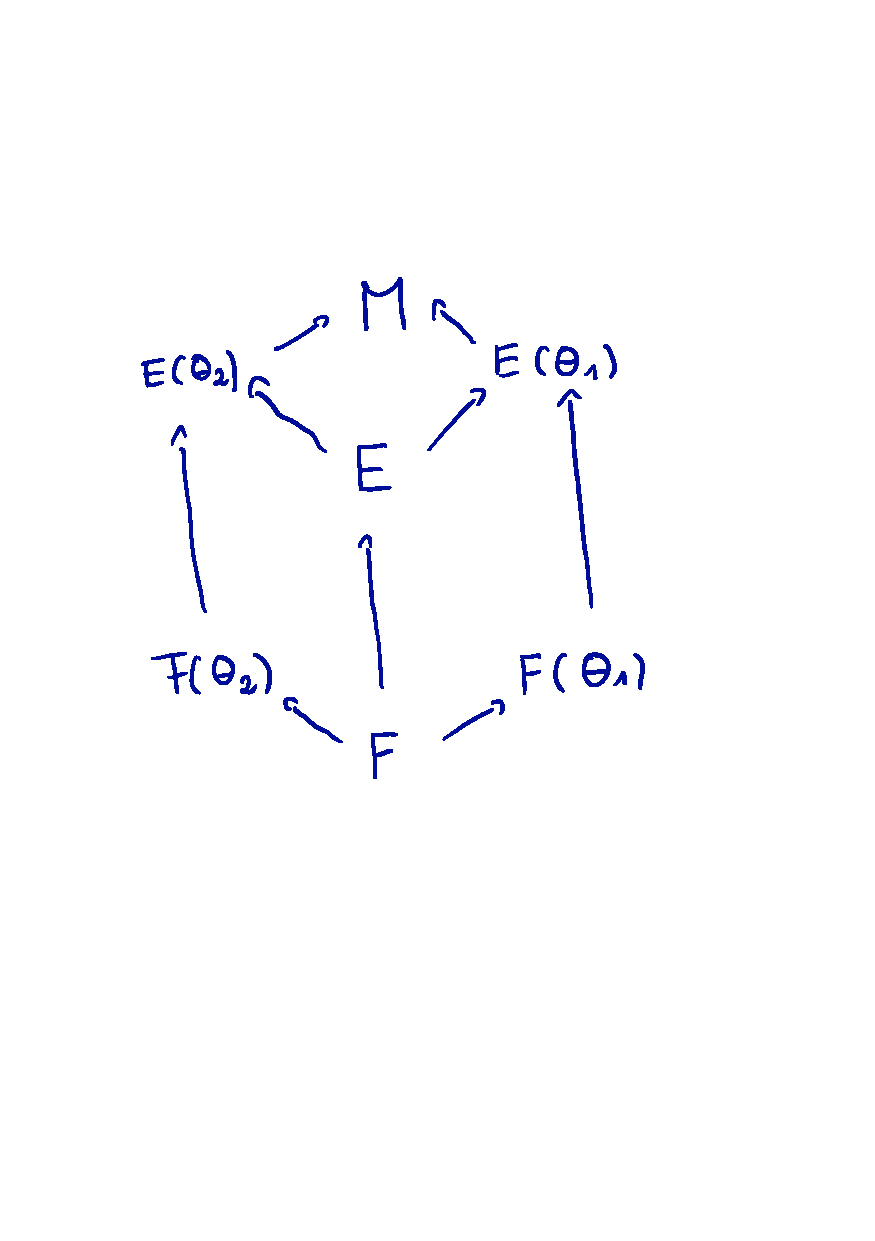
\includegraphics{normal.pdf}  
  \caption{Illustration of the proof of Theorem~\ref{thr:20}}
  \label{fig:1}
\end{figure}



\begin{proof}
  Suppose that $E ⊇ F$ is normal and finite. Then $E = F(u_1,\dots,u_k)$. Each minimal polynomial $p_i(x) ∈ F[x]$ splits into linear factors over $E$, one factor being $(x  - u_i)$. This shows that $E$ is the splitting field of $p_1(x) \cdots p_k(x)$.

  For the converse we assume that $E$ is the splitting field of $f(x) ∈F[x]$ and let $p(x) ∈ F[x]$ be an irreducible polynomial that has a root $θ_1$ in $E$.  Let $M$ be a splitting field of $p(x)$ over $E$ and let  $θ_2$ be another root of $p(x)$ in $M$. The fields $F(θ_1)$ and $F(θ_2)$ are isomorphic. The fields $E(θ_1)$ and $E(θ_2)$ are splitting fields of $f(x)$ over $F(θ_1)$ and $F(θ_2)$ respectively. Theorem~\ref{thr:13} shows that the extensions $E(θ_1)⊇F(θ_1)$ and $E(θ_2)⊇F(θ_2)$  are isomorphic and have the same degree. One has
  \begin{displaymath}
    [E(θ_1):F]  =   [E(θ_1):F(θ_1) ] ⋅ [F(θ_1) :F]  
  \end{displaymath}
  and
  \begin{displaymath}
        [E(θ_2):F]  =   [E(θ_2):F(θ_2) ] ⋅ [F(θ_2) :F]. 
  \end{displaymath}
   which proves, $ [E(θ_1):F ] = [E(θ_2):F ]$. On the other hand, one has
   \begin{displaymath}
      [E(θ_1):F ]  =   [E(θ_1):E ] ⋅ [E :F] 
    \end{displaymath}
    and
    \begin{displaymath}
      [E(θ_2):F ]  =   [E(θ_2):E] ⋅ [E :F] 
    \end{displaymath}
  which shows that $[E(θ_1):E ] =[E(θ_2):E]$ and thus that also $θ_2 ∈ E$. 
\end{proof}

Theorem~\ref{thr:20} has a very important consequence. Let $E ⊇F$ be a finite  normal and separable extension. Then, it is a primitive extension  $E = F(u)$ by Theorem~\ref{thr:16}. Furthermore, if $p(x)∈F[x]$ is the minimal polynomial of $u$, then $p(x)$ splits into linear factors in $E$
\begin{displaymath}
  p(x) = (x-u_1) \cdots (x-u_n),
\end{displaymath}
where $u_1=u$ and $u_2,\dots,u_n$ are the other roots pf $p(x)$. 
Theorem~\ref{thr:17} tells us that  $\gal(E:F) = \{ τ_1,\dots,τ_n\}$ where $τ_i$ is the unique $F$-automorphism that maps $u$ to $u_i$. Thus we fully understand the Galois group of a finite normal and separable field extensions, once we get a hold on the primitive element, its minimal polynomial and the other roots of the minimal polynomial as $F$-linear combinations of $1,u,\dots,u^{n-1}$. We will elaborate on this further. 

\section{Group characters and Dedekind's lemma}
\label{sec:group-char-dedek}

\begin{definition}
  \label{def:4}
  Let $G$ be a group and $E$ a field. A group homomorphism $σ:G → E^*$ is called a \emph{character} of $G$ in $E$. A set $\{σ_1,\dots,σ_n\}$ of characters is called \emph{independent'} if for $e_1,\dots, e_n ∈ E$
  \begin{displaymath}
    e_1 σ_1(g) + \cdots + e_n σ_n(g) = 0 \, \text{ for each } g ∈ G 
  \end{displaymath}
  implies $e_1=\cdots=e_n=0$. 
\end{definition}


\begin{lemma}[Dedekind's Lemma]
  \label{lem:3}
  A finite set of distinct characters of a group $G$ in a field $E$ is independent. 
\end{lemma}

\begin{proof}
  Let $\{σ_1,\dots,σ_n\}$ be a set of distinct characters of $G$ in $E$ for which the assertion is to be shown. We proceed by induction on $n$. For $n=1$ one observes that if $u_1 σ_1(g) = 0$ for each $g ∈G$, then $u_1=0$ since $σ_1(g) ≠0$ for each $g ∈G$.

  For  $n>1$, let $e_1,\dots,e_n ∈E$ with
  \begin{equation}
    \label{eq:15}
   e_1  σ_1(g) + \cdots + e_n  σ_n(g) = 0 \text{ for each } g ∈G.     
  \end{equation}
 We need to show that all $e_i$ are zero. If one $e_i$ is zero, then, by the induction hypothesis,  all others are zero as well. Assume that that all $e_i$ are non-zero. For  $h ∈G$ one has $σ_i(h⋅ g) = σ_i(h) ⋅σ_i(g)$  and clearly
 \begin{equation}
   \label{eq:16}
   e_1  σ_1(h) σ_1(g) + \cdots + e_n  σ_n(h) σ_n(g) = 0 \text{ for each } g ∈G.
 \end{equation}
%
By multiplying~\eqref{eq:15} with $σ_1(h)$ and subtracting  equation~\eqref{eq:16} from the result one obtains 
\begin{displaymath}
   e_2  (σ_1(h) - σ_2(h))   σ_2(g) + \cdots + e_n  (σ_1(h) - σ_n(h))  σ_n(g) = 0 \text{ for each } g ∈G.
 \end{displaymath}
 By the induction hypothesis and the fact that each $e_i$ is non-zero, this means that
 \begin{displaymath}
    (σ_1(h) - σ_i(h)) \, ∀ i∈\{2,\dots,n\}, \ h ∈G 
  \end{displaymath}
  and thus that the characters are all equal, contrary to the assumption that they are distinct.
\end{proof}


\begin{theorem}
  \label{thr:21}
  Let $E ⊇F$ be a finite field extension and denote $\gal(E:F)$ by $G$. One has
  \begin{displaymath}
    |G| ≤ [E:F]. 
  \end{displaymath}
\end{theorem}
\begin{proof}
  Let $[E:F] = n$, $v_1,\dots,v_n ∈E$ be an $F$-basis of $E$ and suppose that there are $n+1$ distinct $F$-automorphisms $σ_0,\dots,σ_n ∈ G$. These are also characters from the group $E^*$ into $E$ and this means that they are independent. Consider the matrix
  \begin{displaymath}
    A =
    \begin{pmatrix}
      σ_0(v_1) & σ_1(v_1) &  \cdots & σ_n(v_1) \\
      σ_0(v_2) & σ_1(v_2) &  \cdots & σ_n(v_2) \\
      \vdots &           &         & \vdots \\
       σ_0(v_n) & σ_1(v_n) &  \cdots & σ_n(v_n) \\
    \end{pmatrix} ∈ E^{n ×n+1}. 
  \end{displaymath}
  There exists a nonzero vector $(x_0,\dots,x_{n})^T ∈E^{n+1}$ which is in the kernel of this matrix. In particular, one has
  \begin{equation}
    \label{eq:17}
    y^T A x = 0 \text{ for each } y ∈ F^{n}. 
  \end{equation}
  The $σ_i$ are $F$-automorphisms and thus 
  \begin{displaymath}
    y^T A = \left( σ_0\left(∑_{i=1}^n y_i v_i\right), σ_1\left(∑_{i=1}^n y_i v_i\right), \dots, σ_1\left(∑_{i=1}^n y_i v_i\right) \right). 
  \end{displaymath}
  Since each element of $E$ is a linear combination of the $v_i$, this, together with~\eqref{eq:17} means that
  \begin{displaymath}
    x_0 σ_0(e)+ \cdots +  x_n σ_n(e) = 0 \text{ for each } e ∈ E. 
  \end{displaymath}
  This is a contradiction, since $x ≠ 0$ and the characters $σ_0,\dots,σ_n$ are independent. Therefore, the assertion follows. 
\end{proof}


Let $σ: E→E$ be a field automorphism. Let us consider the elements of $E$ that are \emph{fixed} by $σ$, i.e., those $e ∈E$ with $σ(e) = e$. These elements are a field, which is quickly verified: Suppose $a$ and $b≠0$ are fixed. Then
\begin{eqnarray*}
  σ(a-b) & = &  σ(a) - σ(b) = a-b\\
  σ(a/b) & = &  σ(a) / σ(b) = a/b.\\   
\end{eqnarray*}
Let $G$ be a group of automorphisms of $E$. The set of elements of $E$ that are fixed by each  $σ ∈G$ is a field, as it is the intersection of all fixed fields of the elements of $G$. We denote this field by $E_G$. 


\begin{theorem}[Dedekind-Artin Theorem]
  \label{thr:25}
  Let $E$ be a field and $G$ be a finite group of automorphisms of $E$, then $E ⊇ E_G$ is a finite extension and 
  \begin{displaymath}
    |G| = [E :E_G]. 
  \end{displaymath}
\end{theorem}
\begin{proof}
  Let $n = |G|$. Assume that there are $n+1$ $E_G$-linear independent elements $u_0,\dots,u_n$ of $E$. We will lead this assumption to a contradiction. This implies the statement, since $|G| ≤ |\gal(E: E_G)| ≤ [E :E_G]$, where the latter inequality is Theorem~\ref{thr:25}.

Consider the following set of $n$ linear equations in $n+1$ variables $x_0,\dots,x_n$
  \begin{equation}
    \label{eq:19}
    σ(u_0) x_0 + \dots +  σ(u_n) x_n = 0,  \, σ ∈G. 
  \end{equation}
This has a nontrivial solution in $E^{n+1}$ and among these solutions let $x^* ∈E^{n+1}$ be a nontrivial solution with  a minimal number $r+1$ of nonzero components. By re-labeling, we can assume that the first $r+1$ components of $x^*$ are non-zero. Furthermore, by multiplying $x^*$ with $1/x^*_0$, we can assume  $x^*_0=1$. This means that 
  \begin{equation}
    \label{eq:21}
     σ(u_0)  + σ(u_1) x^*_1 \dots +  σ(u_n) x^*_r = 0, \, σ ∈G
   \end{equation}
   holds. 
  Since the identity is contained in $G$, one has 
  \begin{equation}
    \label{eq:20}
    u_0 + u_1 x^*_1 + \dots + u_r x^*_r = 0
  \end{equation}
  which implies that one of the $x^*_i$ is not contained in the fixed-field $E_G$. Thus, there exists a $τ ∈ G$ with $τ(x^*_i)≠ x^*_i$. By applying $τ$ to~\eqref{eq:21} we obtain
  \begin{equation}
    \label{eq:22}
     τ(σ(u_0))  + τ(σ(u_1)) τ( x^*_1) + \dots +  τ(σ(u_n))τ( x^*_r) = 0, \, σ ∈G.
   \end{equation}
   and since $τ \circ σ$ runs through the entire group as well, we can re-write~\eqref{eq:22} as
   \begin{equation}
     \label{eq:23}
      σ(u_0)  + σ(u_1) τ( x^*_1) \dots +  σ(u_n) τ( x^*_r) = 0, \, σ ∈G.
    \end{equation}
    Subtracting~\eqref{eq:23} from~\eqref{eq:21} yields
    \begin{equation}
      \label{eq:24}
      σ(u_1) (x^*_1- τ(x^*_1)) +  \dots +  σ(u_n) (x^*_r - τ(x^*_r))= 0, \, σ ∈G.
    \end{equation}
    This is a nontrivial solution to~\eqref{eq:19} with fewer than $r+1$ nonzero components. Namely the solution $y^*$ with
    \begin{displaymath}
      y^*_i =
      \begin{cases}
        (x^*_i- τ(x^*_i)) & 1 ≤ i  ≤ r \\
        0 & \text{ otherwise.}
      \end{cases}
    \end{displaymath}
\end{proof}

\section{Galois extensions}
\label{sec:galois-extensions}


\begin{definition}
  \label{def:5}
  A field extension $E ⊇F$ is called a Galois extension, if $F = E_{\gal(E:F)}$. 
\end{definition}  


\begin{example}
  \label{exe:8}
  The extension $ℂ ⊇ ℝ$ is Galois, since the complex conjugate of any non-real complex number is different from that number. 
\end{example}
 
\begin{example}
  \label{exe:9}
  The extension $ℚ(\sqrt[3]{2}) ⊇ ℚ$ is not Galois, as $\gal(ℚ(\sqrt[3]{2}) : ℚ) = \{id\}$. 
\end{example}


\begin{theorem}
  \label{thr:27}
  
\end{theorem}


Our goal now  is to understand when a finite extension $E ⊇F$ is Galois. We need a refined version of Theorem~\ref{thr:13}.



\begin{theorem}
\label{thr:27}
Let $π: F → \overline{F}$ be an isomorphism of fields and let $f(x) = a_0+ \dots+a_nx^n ∈ F[x]$ be a non-constant separable polynomial.  Let $f^π(x) = π(a_0)+\dots+π(a_n) x^n ∈ \overline{F}[x]$. If $E⊇F$ is a splitting field of $f(x)$ over $F$ and  $\overline{E}⊇\overline{F}$ is a splitting field of $f^π(x)$ over $\overline{F}$, then there exists precisely $[E:F]$ isomorphisms $φ: E → \overline{E}$ that extend $π$, i.e. for which $π(r) = φ(r)$ for each $ r ∈ F$ holds. 
\end{theorem}

The proof is by induction, see diagram below. 

\begin{figure}
  \centering    
\begin{displaymath}
  \begin{CD}
    E @>φ>> \overline{E} \\
    @AAA     @AAA \\
    F(u) @>τ_i >>\overline{F}(v_i) \\
    @AAA     @AAA \\
     F @>π >>\overline{F}
  \end{CD}
\end{displaymath}
\caption{The diagram explaining the proof of Theorem~\ref{thr:27}}
  \label{fig:2}
\end{figure}
\begin{proof}
  First we observe that the mapping $ F[x] → \overline{F}[x]$ with $f ↦ f^π$ is a ring-isomorphism that extends $π$.  Also $p(x) ∈ F[x]$ is irreducible and separable if and only if $p^π(x)∈ \overline{F}[x]$ is irreducible and separable. 

  The proof is by induction on $[E:F]$. If $[E:F] =1$, then $E = F$ and $\overline{E} = \overline{F}$ and $φ = π$ is the only isomorphism from $E$ into $\overline{E}$ that extends $π$.


  If $[E:F] >1$, then there exists an irreducible factor $p(x) ∈F[x]$ of $f(x)$. Let $d$ be the degree of $p(x)$ and  let $u ∈ E$ be a root of $p(x)$. The polynomial $p^π(x)$ is irreducible, separable and of degree $d$ as well. Let $v_1,\dots,v_d ∈ \overline{E}$ be the distinct roots  of $p^π(x)$. For each $i$, there exists a unique isomorphism $τ_i: F(u) → \overline{F}(v_i)$ that extends $π$. For this  $τ_i$ one has  $τ_i(u) = v_i$. Furthermore, the restriction $φ_{|F(u)}$ of an isomorphism $φ:E → \overline{E}$ that extends $π$ is one of these $τ_i$.

  Clearly $f^π(x) = f^{τ_i}(x)$, $E$ is a splitting field of $f(x)$ and $\overline{E}$ is a splitting field of $f^{τ_i}(x)$. By induction, there exist exactly
  \begin{displaymath}
    [E:F(u)] = [E:F] / d
  \end{displaymath}
isomorphisms $φ:E → \overline{E}$ that extend $τ_i$ for each $i$. Since the number of different $τ_i$ to choose from is exactly $d$, this shows that there exist exactly $[E:F]$ isomorphisms $φ:E → \overline{E}$ that extend $π$. 
\end{proof}





\begin{theorem}
  \label{thr:22}
  The following are equivalent for a finite field extension:
  \begin{enumerate}[i)]
  \item  The extension $E ⊇F$ is Galois. \label{item:12}
  \item The extension $E ⊇F$ is normal and separable.\label{item:13}
  \item The field $E$ is the splitting field of a separable polynomial. \label{item:14}
  \end{enumerate}
  A finite field extension $E ⊇F$ is Galois if and only if it is normal and separable. 
\end{theorem}

\begin{proof}
  We begin by showing the implication \ref{item:12}) $⇒$ \ref{item:13}). 
  Suppose that $E ⊇F$ is Galois and let $p(x) ∈F[x]$ be an irreducible polynomial that has a root in $E$. We have to show that $p(x)$ is separable and splits in $E$. To this end, let $u_1,\dots,u_k$ be the different roots of $p(x)$. For an $F$-automorphism $σ$, the elements $σ(u_1),\dots,σ(u_k)$ are the elements $u_1,\dots,u_k$ in a different order. We define the polynomial $g(x)$ as
  \begin{displaymath}
    g(x) = (x-u_1) \cdots (x-u_k) = (x-σ(u_1)) \cdots (x-σ(u_k)) = g^σ(x). 
  \end{displaymath}
  Since $E⊇F$ is Galois, this means that each coefficient of $g(x)$ is in $F$, i.e., $g(x) ∈ F[x]$. But $p(x)$ divides each polynomial in $F[x]$ that has $u_1$ as a root. Since $\deg(p) ≥ \deg(g)$ and since they both are monic, this implies $g = p$. We have shown that $p(x)$ is separable and splits in $E$.

  To see \ref{item:13}) $⇒$ \ref{item:14}), we apply Theorem~\ref{thr:20} and understand that $E$ is the splitting field of a polynomial $f(x) ∈ F[x]$. Each irreducible factor of $f(x)$ is separable, since $E ⊇F$ is a separable extension. Furthermore, the respective root sets of two different monic irreducible factors of $f$ are disjoint (see exercises). Thus, the product $g(x)$  of the distinct monic irreducible factors of $f$ is a separable polynomial. Clearly, $E$ is the splitting field of $g(x)$.

 The implication  \ref{item:14}) $⇒$ \ref{item:12}) follows from Theorem~\ref{thr:27} and the Dedekind Lemma and Theorem~\ref{thr:21}. The Galois group $G = \gal(E:F)$  has cardinality $ |G| = [E:F]$, by Theorem~\ref{thr:27}. Theorem~\ref{thr:21} provides   $[E:E_G] ≥ |G| $ and since $E_G$ is an intermediate field of $E ⊇F$,  we conclude  $E_G = F$, i.e., the extension $E ⊇F$ is Galois. 
  
\end{proof}
%
In fact we also proved the following theorem. 
\begin{theorem}
  \label{thr:24}
  Let $E ⊇ F$ be a finite Galois extension, then $[E:F] = |\gal(E:F)|$. 
\end{theorem}

\begin{proof}
  Let $n = [E:F]$.  The extension $E⊇F$ is primitive, $E = F(θ)$. Let $p(x) ∈ F[x]$ be the minimal polynomial of $θ$ and let $θ=θ_1,\dots,θ_n ∈ E$ be the other roots of $p(x)$. They are all different (separable) and in $E$ (normal).  Theorem~\ref{thr:17} implies  that
\begin{displaymath}
  \gal(E:F) = \{ τ_1,\dots,τ_n\},
\end{displaymath}
 where $τ_i$ is the unique $F$-automorphism that maps $θ$ to $θ_i$. 
\end{proof}

\section{The Galois Correspondence}
\label{sec:galo-corr}

Let $E ⊇ F$ be a field extension with Galois group $G$. The Galois correspondence is a correspondence between the \emph{intermediate fields} $E ⊇ K ⊇F$ and the subgroups $H$ of $G$. We denote these sets as follows
\begin{eqnarray*}
  ℱ & = & \{ K :K \text{ field with }  E⊇K⊇F \} \\
  ℋ & = & \{ H : H \text{ subgroup of } G \} \\
\end{eqnarray*}
%
Also, we use the following notation. For $H ∈ ℋ$ we denote $E_H$ by $H^*$ and for $K ∈ℱ$ we denote $\gal(E:K)$  by $K^*$.

\begin{lemma}
  \label{lem:4}
  Let $E ⊇ F$ be a field extension and $ℱ$ and $ℋ$ be defined as above. 
  For $K,L ∈ ℱ$ and $H,I ∈ℋ$ one has
  \begin{enumerate}[i)]
  \item $H ⊆ H^{**}$
  \item  $K ⊆ K^{**}$
  \item  $K ⊆ L$ implies   $K^* ⊇ L^*$ and   $H ⊆ I$ implies  $H^* ⊇ I^*$
  \item $H^{***} = H^*$ and  $K^{***} = K^*$. 
  \end{enumerate}
\end{lemma}

The next lemma prepares to understand the connection between normal subgroups of the Galois group and intermediate fields $E ⊇ K ⊇F$ that are normal extensions of $F$. 
\begin{lemma}
  \label{lem:6}
  Let $E ⊇ F$ be fields and $G = \gal(E:F)$. Then one has the following.
  \begin{enumerate}[i)] 
  \item If $H$ is a normal subgroup of $G$ (we write $H ◁ G$), then \label{item:9}
    \begin{displaymath}
      σ(H^*) ⊆ H^*, \text{ for each } σ ∈ G.
    \end{displaymath}
  \item  If $K$ is an intermediate field with\label{item:10}
    \begin{displaymath}
       σ(K) ⊆ K, \text{ for each } σ ∈ G,
     \end{displaymath}
     then $K^*◁ G$ and
     \begin{displaymath}
       G / K^* ≡ \{ ρ ∈ \gal(K:F) :ρ \text{ extends to an automorphism of } E\}. 
     \end{displaymath}     
  \end{enumerate}
\end{lemma}
\begin{proof}
  To show~\ref{item:9}) we need to verify that $σ(u) ∈ E_H$ for each $σ ∈ G$. Since $H ◁ G$ one has $σ^{-1} ○ τ ○ σ ∈ H$ for each $τ ∈ H$. This implies
  \begin{displaymath}
    (σ^{-1} ○ τ ○ σ ) (u) = u \text{ for each } u ∈E_H
  \end{displaymath}
  and thus that
  \begin{displaymath}
    τ(σ(u)) = σ(u)  \text{ for each } u ∈E_H. 
  \end{displaymath}
  In other words $σ(E_H) ⊆ E_H$.

  For~\ref{item:10}) we observe that, for each $σ ∈G$,  the restriction $σ_{|K}$ is an $F$-automorphism of the extension $K ⊇F$. The mapping $φ:G → \gal(K:F)$ with $φ(σ) = σ_{|K}$ is a group homomorphism. The kernel consists exactly of $K^* = \gal(E:K)$.
Theorem~\ref{thr:13} shows that each element of $\gal(K:F)$ can be extended to an element of $\gal(E:F)$, which means that $φ$ is surjective. 
  The assertion now  follows from the group-isomorphism theorem. 
\end{proof}

% \begin{lemma}
%   \label{lem:5}
%   Let $E ⊇ F$ be a Galois extension and $E ⊇ K ⊇F$ be an intermediate field. Then $E ⊇ K$ and $K ⊇ F$ are Galois extensions. 
% \end{lemma}

% \begin{proof}
%   The extensions $E ⊇K$ and $K ⊇ F$ are separable. The extension $K ⊇ F$ is separable, by definition.  The extension $E ⊇K$ is separable  because the minimal polynomial of an element $α ∈ E$ over $K$ divides the minimal polynomial of $α$ over $F$.

%   The extension $E ⊇K$ is normal, since it remains to be a splitting field of a polynomial $f(x) ∈ F[x] ⊆ K[x]$.
  
% \end{proof}

\begin{theorem}[Fundamental theorem of Galois theory] 
  \label{thr:23}
  Let $E ⊇F$ be a finite Galois extension of degree $n$ and $ℱ$ and $ℋ$ be defined as above. Then
  \begin{enumerate}[i)]
  \item For each $K ∈ℱ$ one has $K^{**} = K$. \label{item:4}
  \item For each $H ∈ ℋ$ one has $H^{**} = H$. \label{item:5}
  \item For $K ∈ ℱ$ one has \label{item:6}
    \begin{displaymath}
      [E : K ]  =  | K^*|
    \end{displaymath}
      and 
      \begin{displaymath}
        [ K \colon F ]  =  n / |K^*|                 
      \end{displaymath}
  \item For $K ∈ ℱ$ the extension $K ⊇ F$ is normal, if and only if $K^*$ is a normal subgroup of $\gal(E:F)$. \label{item:7}
  \item If $K ⊇F$, $K ∈ ℱ$ is a normal extension, then \label{item:8}
    \begin{displaymath}
      \gal(K:F) ≅ \gal(E:F) / K^*. 
    \end{displaymath}
  \end{enumerate}
\end{theorem}



\begin{proof}
  We first note that, for each intermediate field $K$, the extension $E⊇ K$ is normal and separable, i.e., Galois. This is straightforward and was shown in the exercises.

For~\ref{item:4}), we apply Theorem~\ref{thr:22} and observe $E_{\gal(E:K)} = K$. In other words, the fixed field of the Galois group of $E⊇K$ is $K$ itself.  This is precisely the statement $K^{**} = K$.

Also,   $|K^*|$ is equal to the degree of the extension $[E:K]$ by Theorem~\ref{thr:24} and $[K:F] = n / |K^*|$ follows from the tower law.  This is \ref{item:6}).

We next show~\ref{item:5}). Recall that $H^* = E_H = \{e ∈ E:σ(e) = e \text{ for each } σ ∈ H\}$ and that $H^{**} = \gal(E:E_H)$. The extension $E ⊇ E_H$ is Galois. Theorem~\ref{thr:24} implies
\begin{equation}
  \label{eq:18}
  |H^{**}| = [E:E_{H}]. 
\end{equation}
The Dedekind-Artin Theorem states
\begin{displaymath}
  |H| = [E:E_H].
\end{displaymath}
As  $H^{**} ⊇ H$ this means $H^{**} = H$. 

We next show  \ref{item:7}). Let $K ⊇ F$ be a normal extension. Since it is also separable, one has $K = F(α)$ for some $α ∈K$. The minimal polynomial $p(x) ∈ F[x]$ of $α$ splits in $K$ and any $σ ∈ \gal(E:F)$ carries $α$ to another root of $p(x)$. This means that $σ(K) ⊆ K$ for each $σ ∈ \gal(E:F)$. Lemma~\ref{lem:6}~\ref{item:10}) implies $K^* ◁ \gal(E:F)$.

On the other hand, if $K^*◁ \gal(E:F)$, then Lemma~\ref{lem:6}~\ref{item:9}) shows $σ(K^{**}) = K^{**}$. Since $K^{**} = K$ by \ref{item:4}) of this theorem, one has $σ(K) = K$. The field $K$ is a simple extension, i.e., $K = F(α)$. Each $σ ∈ \gal(E:F)$ carries $α$ to another root of the minimal polynomial $p(x) ∈F[x]$ of $α$ which is, by assumption, an element of  $K$. This means that $p(x)$ splits in $K = F(α)$. In other words, $K ⊇F$ is normal by Theorem~\ref{thr:20}.

Finally,~\ref{item:8}), follows from Lemma~\ref{lem:6}~\ref{item:10}) once we show that each $τ∈ \gal(K:F)$ extends to an automorphism of $E$. But this follows from~Theorem~\ref{thr:13}.

\end{proof}

As a first application, we now describe the intermediate fields  of the extension  $E = \mathrm{GF}(p^n) ⊇ ℤ_p$. In Example~\ref{exe:5}, we developed   $\gal(E:ℤ_p) ≅ C_n$.

\begin{corollary}
  \label{co:2}
  Consider the extension $E = \mathrm{GF}(p^n) ⊇ ℤ_p$. The intermediate fields are precisely the $\mathrm{GF}(p^m)$, where $m$ divides $n$. 
\end{corollary}

\begin{proof}
Let $m$ be a divisor of $n$. The cyclic group   $C_n$ has precisely one subgroup of order $m$. Since $E ⊇ℤ_p$  is Galois, the Galois correspondence shows that there is precisely one intermediate field of order $n/m$, for each divisor $m$ of $n$. 
\end{proof}


%%% Local Variables:
%%% mode: latex
%%% TeX-master: "notes"
%%% End:
 
 \chapter{Applications}
\label{cha:applications}


\section{Insolvability of polynomials}
\label{sec:insolv-polyn}

In this section, we will show a connection between the Galois group of a polynomial and the solvability of a polynomial in radicals.

\begin{definition}
  \label{def:6}
  Let $f(x) ∈ F[x]$ be a polynomial, where $F$ is a field. The \emph{Galois group} of  $f(x)$ is $\gal(E:F)$, where $E$ is a splitting field of $f(x)$. 
\end{definition}

This definition makes sense because if $E'$ is another splitting field of $F$, then $E$ and $E'$ are isomorphic and therefore, also $\gal(E:F)$ and $\gal(E':F)$ are isomorphic. (Exercise)


\begin{definition}
  \label{def:7}
  A field extension  $E ⊇F$  is called \emph{radical extension}, if a chain of intermediate fields  $E = E_0 ⊇ E_1 ⊇ \cdots ⊇ E_n = F$ exists, such that
  \begin{displaymath}
    E_i = E_{i+1}(u_i), \text{ where } u_i^{n_i} ∈ E_{i+1} \text{ for some } n_i≥1. 
  \end{displaymath}
  A polynomial $f(x) ∈F[x]$ is called \emph{solvable} if some radical extension of $f(x)$ contains a splitting field of $f(x)$. 
\end{definition}
Thus, if a polynomial is solvable, then each of its roots can be written as a nested finite  expression involving elements of $F$, addition, subtraction, multiplication and division, as well as taking $n$-th roots.
A rational polynomial of degree at most $4$ is solvable. 
Our goal is to show that there exists a  polynomial $f(x) ∈ℚ[x]$ of degree $5$ that is not solvable. 
%
We next recall the definition and some characterization of a solvable group. 
\begin{definition}
  \label{def:8}
  A group  $G$ is \emph{solvable} if there exists a chain of subgroups
  \begin{displaymath}
    G = G_0 ⊇ G_1 ⊇ \cdots ⊇ G_n = \{1\}
  \end{displaymath}
  such that
  $G_{i+1} ◁ G_i$ and $G_i / G_{i+1}$ is abelian for each $1≤i <n$. 
\end{definition}

\begin{lemma}
  \label{lem:7}
  If $G$ is a group and $K ◁ G$, then $G$ is solvable if and only if $K$ and $G/K$ are solvable. 
\end{lemma}

We will show the if direction of the Galois criterion. This will enable us to show that a certain polynomial is not solvable by showing that its Galois group is not solvable. 
\begin{theorem}[Galois criterion] 
  \label{thr:26}
  Let $F$ be a field of characteristic zero and $f(x) ∈ F[x]$. The Galois group of $f(x)$ is solvable if and only if $f(x)$ is a solvable polynomial. 
\end{theorem}
The group $S_5$ is not solvable. We will construct a polynomial of degree $5$ in $ℚ[x]$ whose Galois group is $S_5$.

\begin{lemma}
  \label{lem:8}
  If $p$ is a prime number, then $S_p$ is generated by any $2$-cycle, together with any $p$-cycle. 
\end{lemma}


\begin{proof}
  We assume that the $p$-cycle is $ σ= (1,2, \dots,p)$ and the $2$-cycle is $τ=(1,k)$. Now $σ^{k-1}$ is  a $p$-cycle as well that maps $1$ to $k$. Therefore, we may assume that $ σ= (1,2,\dots,p)$ and $τ = (1,2)$. We have $(k+1,k+2) = σ^k τ σ^{-k}$. Since $(1,a+1) = (1,a) (a,a+1)(1,a)$ it follows that, for each $a$,  $(1,a)$ is in the subgroup generated by $τ$ and $σ$. The transpositions $(1,a)$ generate $S_p$. 
\end{proof}

\begin{example}
  \label{exe:10}
  The polynomial $p(x) = x^5 - 6x +2 ∈ ℚ[x]$  is not solvable. First of all, we note that $p(x)$ is irreducible (Eisenstein). Let $E$ be the splitting field of $p(x)$. The Galois group $G =\gal(E:ℚ)$ is isomorphic a subgroup of the permutations of the roots $X ⊆ ℂ$ of $p$.

  The polynomial $p(x)$ has three distinct real roots. This can be seen by inspecting the real roots of the derivative $p'(x) = 5x^4 -6$, which are $\pm \sqrt[4]{6/5}$. The polynomial is positive at $-\sqrt[4]{6/5}$ and negative at $\sqrt[4]{6/5}$. The other two non-real roots are complex conjugates of each other. Convex conjugation is in $G$, it is a transposition of the complex roots.

  Since $E⊇ ℚ$ is Galois, we have $ |G| = [E:ℚ]$. Since $p$ is irreducible and of degree $5$, we have that $5$ divides $G$ and thus there exists an element of order $5$ in $G$ by Cauchy's Theorem. The only elements of order $5$ in $S_5$ are the $5$-cycles. Thus, by Lemma~\ref{lem:8}, $G$ is isomorphic to $S_5$ and thus not solvable. By the Galois criterion, $p(x)$ is not solvable. 
\end{example}


We will now prepare for the proof of the \emph{if} direction of the Galois criterion, namely, if $f(x)$ is solvable, then its Galois group is a solvable group.

\begin{lemma}
  \label{lem:9}
  If $G$ is a cyclic group of order $n$, then $\mathrm{aut}(G)≅ ℤ_n^*$. 
\end{lemma}

\begin{proof}
  Since $G$ is isomorphic to $(ℤ_n,+)$ we only have to show $\mathrm{aut}(ℤ_n)≅ ℤ_n^*$. Let $σ:ℤ_n →ℤ_n$ be an automorphism and let $σ(1) = m$. Clearly, $m$ has to be a generator of $ℤ_n$ and this is the case if and only of $\gcd(n,m)=1$. On the other hand,  each $σ_m: ℤ_n → ℤ_n$ with $σ(a) = a ⋅m$  and $\gcd(n,m)=1$ is an automorphism. This shows that the mapping $τ: ℤ_n^* →\mathrm{aut}(ℤ_n)$ with $τ(m) = σ_m$ is an isomorphism of groups.  
\end{proof}

Let $E ⊇F$ be a field extension. An element  $ω ∈ E$ is a \emph{primitive $n$-th root of unity over $F$} if it is a root of $x^n -1$ and if its order is $n$. 

\begin{theorem}
  \label{thr:28}
  If $F$ is a field and $n≥1$ is an integer, then a primitive $n$-th root of unity $ω$ over $F$ exists if and only if $\car(F)$ does not divide $n$. In this case,
  \begin{enumerate}[i)]
  \item $F(ω)$is the splitting field of $x^n-1$ over $F$. \label{item:11} 
  \item $F(ω) ⊇ F$ is a finite Galois extension and $\gal(F(ω):F)$ is \label{item:15} isomorphic to a subgroup of $ℤ_n^*$. 
  \end{enumerate}
\end{theorem}

\begin{proof}
  If $p = \car(F) | n$, then consider the polynomial
  \begin{displaymath}
    x^n - 1 = (x^{n/p} -1)^p. 
  \end{displaymath}
  If a primitive $n$-th root of unity  would $ω$ would exist, then $1,ω,\dots,ω^{n-1}$ are n different roots of $x^{n/p} -1$ which is impossible, since the degree of this polynomial is less than $n$.

  If $p$ does not divide $n$, then consider the polynomial
  \begin{displaymath}
    x^n -1. 
  \end{displaymath}
  The derivative of this polynomial is $n x^{n-1}$ and this is not equal to zero since $p$ does not divide $n$. The greatest common divisor of $n x^{n-1}$ and $x^n -1$ is one and, by  Theorem~\ref{thr:14}, $x^n-1$ has multiple roots. Let $E ⊇F$ be a splitting field of $x^n-1$.  The roots $G = \{ r ∈ E :r^n =1\}$ are a subgroup of $E^*$. Each finite subgroup of the units in a field is cyclic. The generator $ω ∈ G$ with $〈 ω 〉 = G$ is a primitive $n$-th root of unity.

The assertion~\ref{item:11}) is immediate. Since $x^n-1$ is separable, \ref{item:11}) together with Theorem~\ref{thr:22}) implies that $F(ω) ⊇F$   is Galois. By restriction to $\{1,ω,\dots, ω^{n-1}\}$, each $σ ∈ \gal(F(ω) :F)$ is an automorphism of the cyclic (multiplicative) group $\{1,ω,\dots, ω^{n-1}\}$. This, together with Lemma~\ref{lem:9} shows that $\gal(F(ω) :F)$ is isomorphic to a subgroup of $ℤ_n^*$.   
\end{proof}


\begin{theorem}
  \label{thr:29}
  Let $F$ be a field containing a primitive $n$-th root of unity and consider an extension $F(u) ⊇ F$,where $u^n ∈ F$. Then $F(u) ⊇ F$ is a Galois extension and $\gal(F(u):F)$ is abelian. 
\end{theorem}

\begin{proof}
  Let $ω$ be a primitive $n$-th root of unity and let $u^n = a ∈ F$. The polynomial $f(x) = x^n -a$ has $n$ distinct roots $u, ωu, \dots, ω^{n-1} u$. Since the minimal polynomial $p(x)∈ F[x]$  of $u$ divides $f(x)$ this shows that $p(x)$ is separable and splits in $F(u)$. This means that $F(u)$ is a normal and separable extension of $F$ and thus that $F(u) ⊇ F$ is Galois. Each $F$-automorphism of $F(u)$ is uniquely specified by the image of $u$ which is a root of $p(x)$ and thus of the form $ω^i u$ for some $i ∈ \{0,\dots,n-1\}$. We denote the element of $\gal(F(u):F)$ that maps $u$ to $ω^i u$ by $τ_i$. For two roots  $ω^iu$ and $ω^ju$ of $p(x)$ one has 
  \begin{eqnarray*}
    (τ_i \circ τ_j ) (u) & = & τ_i(  ω^ju ) \\
                         & = &  ω^jτ_i( u ) \\
                         & = & ω^{j+i} u \\
                         & = & ω^{i+j} u \\
                         & = &  ω^iτ_j( u ) \\
                         & = &  τ_j( ω^iu ) \\
                         & = & (τ_j \circ τ_i ) (u).
  \end{eqnarray*}
  This shows that $\gal(F(u) :F)$ is abelian. 
\end{proof}


\begin{theorem}
  \label{thr:30}
  Let $E ⊇F$ be a radical Galois extension, where $\car(F) = 0$, then  $\gal(E:F)$ is a solvable group. 
\end{theorem}

\begin{proof}
  We find an extension $K ⊇ E ⊇ F$ such that
  \begin{enumerate}[a)]
  \item $K ⊇F$ is Galois and,
  \item $\gal(K:F)$ is solvable. 
  \end{enumerate}
  This will be sufficient since Theorem~\ref{thr:23}~\ref{item:8}) implies
  \begin{displaymath}
    \gal(E:F) ≅ \gal(K:F) / \gal(K:E)  
  \end{displaymath}
  and in particular $\gal(E:F)$ is a homomorphic image of $\gal(K:F)$. And the homomorphic image of a solvable group is again a solvable group.

  To this end let
  \begin{displaymath}
    E = E_0 ⊇E_1 ⊇ \cdots ⊇ E_r = F
  \end{displaymath}
  be a tower of intermediate fields with $E_i = E_{i+1}(u_i)$ and $u_i^{n_i} ∈ E_{i+1}$ for $i=0,\dots,r-1$. Let $n = n_1\cdots n_{r-1}$ and let $ω$ be a primitive $n$-th root of unity, which exists, since $\car(F) = 0$. Define $K_i = E_i(ω)$ for $i=0,\dots,r$. Let
  \begin{equation}
    \label{eq:25}
    K = K_0 ⊇ K_1 ⊇ \cdots K_r ⊇K_{r+1} = F
  \end{equation}
  be the corresponding chain of intermediate fields. Inspect the extensions  $K_i ⊇ K_{i-1}$ for $i=i,\dots,r-1$.   We have  $K_i = K_{i+1}(u_i)⊇ K_{i+1}$ with  $u_i^{n_i} ∈ K_{i+1}$ and   $ K_{i+1} $ contains a primitive $n_i$-th root of unity. Thus $K_i ⊇ K_{i-1}$ is Galois with an abelian Galois group by Theorem~\ref{thr:29}. Also $K_r ⊇ K_{r+1}$ is Galois with an abelian Galois group by Theorem~\ref{thr:28}. Now consider the chain of subgroups of $\gal(K :F)$
  \begin{equation}
    \label{eq:26}
    \{ id\} = \gal(K:K_0) ⊆  \gal(K:K_1) ⊆ \cdots ⊆ \gal(K:K_r) ⊆ \gal(K:K_{r+1}).  
  \end{equation}
  The fundamental theorem gives
  \begin{enumerate}[i)]
  \item $\gal(K:K_i) ⊲ \gal(K:K_{i+1})$  by Theorem~\ref{thr:23}~\ref{item:7}), and
    \item $\gal(K_i : K_{i+1}) ≅ \gal(K : K_{i+1}) / \gal(K:K_i)$ by Theorem~\ref{thr:23}~\ref{item:8}). In particular, $\gal(K : K_{i+1}) / \gal(K:K_i)$ is abelian. 
  \end{enumerate}
This shows that $\gal(K:F)$ is solvable. 
  
\end{proof}

\section{A Galois extension whose Galois group is ismorphic to $S_n$}
\label{sec:galo-extens-whose}

Let $F$ be a field and 
$F[x_i] = F[x_1,\dots,x_n]$  be the polynomial ring in indeterminants $x_1,\dots,x_n$.  A polynomial $f(x) ∈F[x_i]$ is \emph{symmetric} if
\begin{displaymath}
  f(x_1,\dots,x_n) = f(x_{σ_1},\dots,x_{σ_n}) \, \, \text{ for each } σ ∈S_n. 
\end{displaymath}
The \emph{elementary symmetric polynomials} $s_0,\dots,s_n ∈ F[x_i]$  are defined as follows
\begin{eqnarray*}
  s_0 & = & 1 \\
  s_k & = & ∑_{i_1<i_2< \cdots < i_k} x_{i_1}x_{i_2} \cdots x_{i_k} \, \text{ for } k=1,\dots,n. 
\end{eqnarray*}
One has the formula
\begin{displaymath}
  (x-u_1) \cdots (x- u_n) = ∑_{i=0}^n (-1)^i s_i(u_1,\dots,u_n) x^i. 
\end{displaymath}

Let $E = F(x_1,\dots,x_n)$ be the field of fractions of $F[x_1,\dots,x_n]$. An element $r(x_1,\dots,x_n) = f(x_1,\dots,x_n) / g(x_1,\dots,x_n)$  with $g ≠0$ is called a \emph{symmetric rational form} if $r(x_{σ_1},\dots,x_{σ_n}) = r(x_1,\dots,x_n)$ holds for each $σ ∈S_n$.

Each element $σ ∈S_n$ can be mapped to a corresponding element $σ' ∈ \gal(E:F)$, where $σ'(r(x_1,\dots,x_n))  =  r(x_{σ_1},\dots,x_{σ_n})$. This mapping is a one-to-one group homomorphism. Let $S⊆E$ be the subfield of symmetric rational forms and let $G = \{ σ' :σ ∈S_n\}$ be the subgroup of $\gal(E:F)$ 


\begin{theorem}
  \label{thr:31}
  Let $F$ be a field, $E = F(x_1,\dots,x_n)$ and $S ⊆E$ be the subfield of all symmetric rational forms.
  \begin{enumerate}[i)]
  \item $E ⊇S$ is Galois, $[E:S] = n!$ and $\gal(E:S) ≅ S_n$.
\item $S = F(s_0,\dots,s_n)$ and $E$ is the splitting field of the polynomial
  \begin{displaymath}
    f(t) = t^n - s_1 t^{n-1} + s_2 t^{n-2} + \dots + (-1)^n s_n 
  \end{displaymath}
  over $S$. 
  \end{enumerate}
\end{theorem}

\begin{proof}
  The field $S$ is the fixed field of the group $G$. The Dedekind-Artin Theorem (Theorem~\ref{thr:25}) shows 
  \begin{displaymath}
    [E:S ] =|G| = n!.  
  \end{displaymath}

  
  The polynomial $f(t) ∈ F(s_0,\dots,s_n)$ splits as
  \begin{displaymath}
    f(t) = (t - x_1) \cdots (t-x_n)  ∈ S[x_1,\dots,x_n]
  \end{displaymath}
  in $E$. Clearly  $E$ is the splitting field
  of $f(t)$ over $F(s_0,\dots,s_n)$. This shows that $[E:F(s_0,\dots,s_n)] ≤n!$ and since $F(s_0,\dots,s_n) ⊆S$ also that $S = F(s_0,\dots,s_n)$. 

  Since $f(t)$ is separable,   $E ⊇S$ is Galois.  Also  $\gal(E:S) ⊇ G ≅S_n$ but with Theorem~\ref{thr:21} $|\gal(E:S) | ≤ [E:S] = n! = |G|$ and thus $\gal(E:S)  = G ≅S_n$. 
\end{proof}



\section{Finite Galois extensions with solvable Galois groups}
\label{sec:finite-galo-extens}

In this section, we assume throughout that the characteristic of $F$ is zero.




\begin{theorem}
  \label{thr:32}
  Suppose that $E ⊇F$ is a Galois extension with $\gal(E:F) ≅ ℤ_p$ with a prime $p$. If $F$ contains a primitive $p$-th root of unity, then there exists an $α ∈E$ such that $E = F(α)$ and $α^p ∈F$.
\end{theorem}

\begin{proof}
  Let $σ$ be a generator of $\gal(E:F)$, let $ω ∈F$ be a primitive $p$-th root of unity  and let $β ∈ E ⧹F$.  For $i=0,\dots,p-1$ we define the $i$-th Lagrange resolvent
  \begin{displaymath}
    α_i = β + ω^{-i} σ(β) + ω^{-2i} σ^2(β) + \cdots + ω^{-(p-1)i} σ^{(p-1)}(β) 
  \end{displaymath}
  One has
  \begin{displaymath}
    σ(α_i) = ω^i α_i
  \end{displaymath}
  and thus
  \begin{displaymath}
    σ(α_i^p) = α_i^p. 
  \end{displaymath}
  This implies that $α_i^p∈F$ and $α_i \notin F$ if $a_i ≠0$ and $i≥1$.  Thus, in the latter case $F(α_i) = E$ with $α_i^p ∈F$ would follow.
  We next show that at least one of the $α_i ≠ 0$ where $i=\{1,\dots,p-1\}$.

  First observe that $σ(α_0) = α_0$ and thus $α_o ∈F$. If $α_1=α_2 = \cdots = α_{p-1} = 0$, then
  \begin{eqnarray*}
    α_0 & = & α_0 + α_1 + \cdots + α_{p-1} \\
        & = & pβ + ∑_{i=1}^{p-1} ∑_{j=0}^{p-1} ω^{-i j} σ^i(β) \\
        & = & pβ,
  \end{eqnarray*}
  since $∑_{j=0}^{p-1} ω^{-i j} =0$ for $i=1,\dots,p-1$. This implies $β = α_0 / p$ which is a contradiction to $β ∈ E ⧹F$. 
\end{proof}


\begin{theorem}
  \label{thr:33}
  Let $E ⊇F$ be a finite Galois extension and suppose that $F$ has a
  primitive $p$-th root of unity for each prime number that divides
  $|\gal(E:F)|$. If $\gal(E:F)$ is solvable, then $E ⊇F$ is a
  radical extension. 
\end{theorem}
\begin{proof}
  In the exercises you show that a finite group $G$ is solvable if and only if there are subgroups
   \begin{displaymath}
    \{1\} = G_n ⊆G_{n-1}⊆ \cdots ⊆ G_1 ⊆G_0 = G  
  \end{displaymath}
  such that
  \begin{enumerate}[a)]
  \item $G_i$ is normal in $G_{i-1}$
  \item $|G_{i-1}| : |G_i|$ is a prime.
  \end{enumerate}

  Let $E_{G_i}$ be the fixed field of the corresponding chain of the Galois group $G = \gal(E:F)$, i.e., we have
  \begin{displaymath}
    E = E_{G_n} ⊇ E_{G_{n-1}} ⊇ \cdots ⊇ E_{G_1} ⊇ E_{G_0} = F.
  \end{displaymath}
  We can apply Theorem~\ref{thr:32} once we have shown that
  \begin{enumerate}[i)]
  \item $E_{G_i} ⊇ E_{G_{i-1}}$ is Galois for each $i∈\{n,\dots,1\} $and \label{item:16}
  \item $[E_{G_i}: E_{G_{i-1}}]$ is a prime dividing $[E:F] = |\gal(E:F)|$. \label{item:17}
  \end{enumerate}

  By the main Theorem~\ref{thr:23}~\ref{item:7}) we  have that $E_{G_{1}} ⊇ E_{G_{0}}=F$ is Galois since $G_1 ⊲ G$. The extension $E = E_{G_n} ⊇ E_{G_1}$ is Galois with Galois group $G_1$. We have $G_2 ⊲ G_1$ and again by the main theorem we have $ E_{G_2} ⊇  E_{G_1}$ is Galois. Again the extension $ E_{G_n} ⊇  E_{G_2}$ is Galois with Galois group $G_2$. Continuing in this way, we see that~\ref{item:16}) holds. 

  By the main Theorem~\ref{thr:23}~\ref{item:8}) we have
  \begin{displaymath}
    \gal(E_{G_i} :  E_{G_{i-1}}) ≅ {G_{i-1}} / {G_i} 
  \end{displaymath}
  which shows that the index $[E_{G_i} :  E_{G_{i-1}}]$ is a prime. Notice that $[E_{G_i}: E_{G_{i-1}}]$ divides $[E:F] = |\gal(E:F)|$ by the tower law.  This shows \ref{item:17})  
\end{proof}


We now are able to prove the missing direction of the Galois criterion. You will be asked for a proof of this theorem in the exercises.

\begin{theorem}
  \label{thr:34}
  Let $E ⊇F$ be a finite Galois extension with $\car(F) = 0$ and let $ω$ be a primitive $m$-th root of unity, where $m = [E:F]$. If $\gal(E:F)$ is solvable, then $E(ω) ⊇ F$ is a radical extension. 
\end{theorem}



%%% Local Variables:
%%% mode: latex
%%% TeX-master: "notes"
%%% End:
 
 

\bibliographystyle{abbrv}
\bibliography{books}
\end{document}


%%% Local Variables:
%%% mode: latex
%%% TeX-master: t
%%% End:


 